
\documentclass[italian,11pt]{report}		

\usepackage[utf8]{inputenc}
\usepackage[italian]{babel}
\usepackage[T1]{fontenc}
\usepackage{mathtools}
\usepackage{graphicx}


\author{Gianluca Fugante\\ Elisa Radaelli\\ Silvia Zanoli}
\title{ Relazione di laboratorio\\ Effetto Compton}
%\date{}


%%%----------------------------------------------------------
\begin{document}
%%%----------------------------------------------------------
\maketitle	
\tableofcontents
%%%----------------------------------------------------------

\chapter*{Introduzione}

L’esperienza descritta consiste in una verifica sperimentale dell’effetto
Compton utilizzando una sorgente di $\prescript{22}{}{Na}_{}^{}$ che decade $\beta^{+}$. Sfruttando la coincidenza di due fotoni emessi \textit{back-to-back}, è stata verificata la legge che mette in relazione l'energia del fotone scatterato con l'angolo di diffusione ed è stata misurata la sezione d'urto per diversi angoli. Nella prima fase dell'esperienza, sono state determinate le condizioni ottimali per il lavoro, fissando il voltaggio di lavoro, lo shaping-time e calibrando in energia il sistema. Successivamente si è proceduto con le misure vere e proprie: dopo aver scelto come disporre le apparecchiature, sono stati analizzati gli spettri ottenuti a diversi angoli. I dati ricavati ci hanno permesso di verificare la legge Compton e la legge Klein-Nishina. E' stato poi possibile, a partire dai dati ottenuti, misurare il raggio e la massa dell'elettrone.

%%%----------------------------------------------------------
\chapter{Fisica dell'esperimento}
%%%----------------------------------------------------------




I fotoni sono particelle neutre di massa nulla che non risentono dell’interazione coulombiana. A differenza delle particelle cariche che interagiscono con la materia principalmente tramite ionizzazione, i fotoni danno vita a tre fenomeni distinti: effetto Compton, produzione di coppie e effetto fotoelettrico. L’importanza relativa dei tre fenomeni è funzione dell’energia del fotone incidente e del numero atomico Z del materiale considerato.  

\vspace{5mm}


\begin{figure}[htp]
\centering
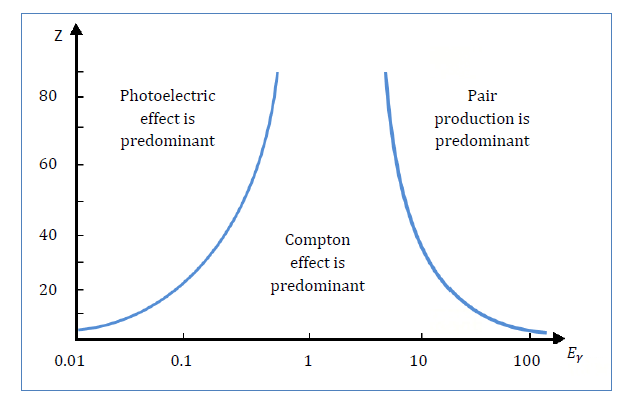
\includegraphics[width=8cm]{cattura46.png}
\caption{Interazione dei fotoni con la materia}
\end{figure}

\vspace{5mm}

Con “effetto Compton” si intende lo scattering elastico di un fotone su un elettrone del materiale. Il fenomeno consiste nel trasferimento di un tetramomento all’elettrone, considerato inizialmente in quiete e libero. Questo determina la diffusione ad un angolo $\theta$ del fotone incidente e il rinculo dell’elettrone.
\vspace{5mm}

\begin{figure}[htp]
\centering
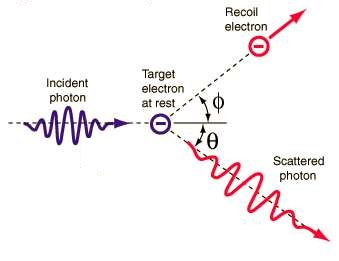
\includegraphics[width=6cm]{compton.jpg}
\caption{Schema dell'effetto Compton}
\end{figure}
\vspace{5mm}

Ciò che caratterizza questo fenomeno è una relazione univoca tra l’angolo di diffusione del fotone incidente e la sua energia dopo l’urto secondo la legge: 
\begin{equation}
\frac{E'}{E} =\frac{1}{1+\frac{E}{m_{e}c^2}(1-cos\theta)}
\end{equation}
dove E rappresenta l’energia del fotone incidente, E’ l’energia del fotone dopo l’interazione e $\theta$ l’angolo di deflessione del fotone. La relazione sopra presentata si ricava imponendo la conservazione del tetramomento nell’interazione.



%%\begin{equation}
\begin{align*}
p_{\gamma}&=(E_{0_\gamma} \hspace{0,5cm} E_{0_\gamma}) &
p'_{\gamma}&=(E_{\gamma} \hspace{0,5cm} E_{\gamma}cos(\theta))\\
p_{e}&=(m_{e} \hspace{0,5cm} 0) &
p'_{e}&=(E_{e} \hspace{0,5cm} \vec{p_{e}})\\
\end{align*}
%%\end{equation}
dove $p_{\gamma}$ e $p'_{\gamma}$ rappresentano il tetramomento del fotone prima e dopo l'urto mentre $p_{e}$ e $p'_{e}$ rappresentano il momento dell'elettrone. Si impone quindi $$p_{\gamma}+p'_{\gamma}=p_{e}+p'_{e}$$ e si ricava la relazione (1.1).
%%%----------------------------------------------------------
\chapter{Apparato sperimentale}
%%%----------------------------------------------------------

\section{Sorgente}
La sorgente radioattiva utilizzata è un campione di $\prescript{22}{}{Na}_{}^{}$. Questa decade tramite $\beta^{+}$ con una probabilità del 89,90$\%$ in un nucleo eccitato di Ne, con produzione di un positrone e di un neutrino elettronico. Allo stesso livello eccitato del Neon si arriva tramite cattura elettronica con una branching ratio del 10,10$\%$. Il Neon eccitato ${Ne}^{*}$ decade quasi istantaneamente nel livello fondamentale emettendo un fotone da 1274 keV. Nel restante 0,06$\%$ dei casi si ha un ulteriore decadimento $\beta^{+}$ che porta la sorgente di Na direttamente nel ground state di Ne. 



\begin{figure}[htp]
\centering
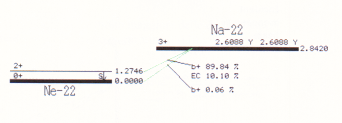
\includegraphics[width=8cm]{decadimentoNa.png}
\end{figure}
Il positrone emesso nei decadimenti $\beta^{+}$ forma uno stato legato con gli elettroni del materiale attraversato, detto positronio. Questo si annichila emettendo due fotoni \textit{back-to-back} che trasportano un'energia di 511keV. Questa proprietà di emissione dei fotoni in direzioni opposte viene sfruttata analizzando il segnale in coincidenza rilevato dai due scintillatori posti lungo la stessa direzione.

\section{Strumentazione}
L'apparato è costituito da due rivelatori inorganici che indicheremo con A (NaI, ioduro di Sodio) e B ($\prescript{}{}{CeBr}_{3}^{}$, bromuro di Cerio). I due rivelatori sono scintillatori, cioè apparecchi in grado di trasformare l'energia di eccitazione del materiale causata dal passaggio del fotone incidente in luce visibile che viene poi fatta convogliare nel fotocatodo di un fotomoltiplicatore, il quale permette di convertire il segnale luminoso in un segnale elettrico. Gli elettroni vengono quindi raccolti sull'anodo da cui viene ricavato il segnale. Per acquisire correttamente il segnale del rilevatore al $\prescript{}{}{CeBr}_{3}^{}$, abbiamo collegato a quest'ultimo un preamplificatore e un amplificatore: il preamplificatore permette di allungare temporalmente il segnale mentre l'amplificatore modifica la forma e lo \textit{shaping-time} (tempo di formazione) del segnale. Gli impulsi in uscita sono stati poi inviati ad un ADC (analizzatore multicanale) che fornisce lo spettro del fenomeno. I due rivelatori sono alimentati separatamente da due generatori di tensione che sono stati regolati nella prima fase dell'esperienza. L'analisi dati è stata effettuata mediante il programma \textit{Maestro} che fornisce un istogramma mettendo in relazione canali (convertiti in energia nella calibrazione dell'apparato) al numero di interazioni rilevate. Tutti i fit presentati sono stati eseguiti con il programma \textit{Root}. Nello studio degli spettri è stato necessario analizzare il fondo ambientale, così da poter distinguere i decadimenti interni al rivelatore e quelli dipendenti da fattori esterni. A tal proposito, in prima approssimazione è stato possibile rimuovere il fondo con una interpolazione lineare di root per poi effetture un'analisi precisa acquisendo dati senza sorgente per circa una settimana.

%%%----------------------------------------------------------     
\chapter{Operazioni Preliminari}
%%%----------------------------------------------------------

Prima di procedere con le misure, è stato necessario definire i parametri ottimali di voltaggio e shaping-time in cui operare. Successivamente è stata effettuata una calibrazione energetica per mettere in relazione i bin individuati con il programma \textit{Mestro} con le energie dei fotoni rilevati.

\section{Tensione di alimentazione}
In questa fase è stato scelto il voltaggio di alimentazione di entrambi i rivelatori. Si studia quindi la dipendenza del numero di interazioni osservate nel picco di 511keV in funzione del voltaggio, a parità di live time. Il voltaggio ottimale è quello per cui l'area sottesa dalla gaussiana rappresentante il picco risulta costante al variare della tensione (\textit{Plateau}). In questo modo si riescono a mantenere le prestazioni del rivelatore approssimativamente indipendenti dalle fluttuazioni del voltaggio nel tempo.
Le misure sono state effettuate variando il voltaggio del rilevatore e acquisendo l'area del fotopicco osservato. Ogni misura è stata della durata di 300s. Le misure sono state analizzate in prima approssimazione con il programma \textit{Maestro} e successivamente con \textit{Root}. Ogni spettro è stato fittato con una gaussiana, che rappresenta il fotopicco a 511kev, e con un polinomio di primo grado, che permette di rimuovere il fondo ambientale. Da qui sono state ricavate le aree delle gaussiane e la relativa incertezza. Abbiamo operato allo stesso modo con i due rilevatori, ottenendo due grafici area($Canali^{2}$)-voltaggio(V).

\newpage
\begin{itemize}
    \item NaI 
   
    Il voltaggio scelto è 750V.
    \vspace{1cm}
    \begin{center}
         \begin{tabular}{cccc}
          \hline
          $\Delta$V(V) & Picco(Ch) & $\sigma_{picco}$(Ch) & Area\\
          \hline\hline
          600& 2392 & 123 &14154$\pm$ 364 \\
          620& 1676 & 97 & 12731$\pm$346 \\
          640& 3841 & 190 & 13171$\pm$379 \\
          660& 4982 & 238 & 13501$\pm$238 \\
          680& 3190 & 164 & 13856$\pm$345 \\
         700& 4206 & 213 & 12528$\pm$386 \\
            720& 4768 & 224 & 13000$\pm$337 \\
           740& 6324 & 287 & 12824$\pm$344 \\
          760& 5486 & 230 & 12926$\pm$248 \\
           780& 6556 & 270 & 12783$\pm$245 \\
         \hline 
          \end{tabular}
    \end{center}
    
\begin{figure}[htp]
\centering
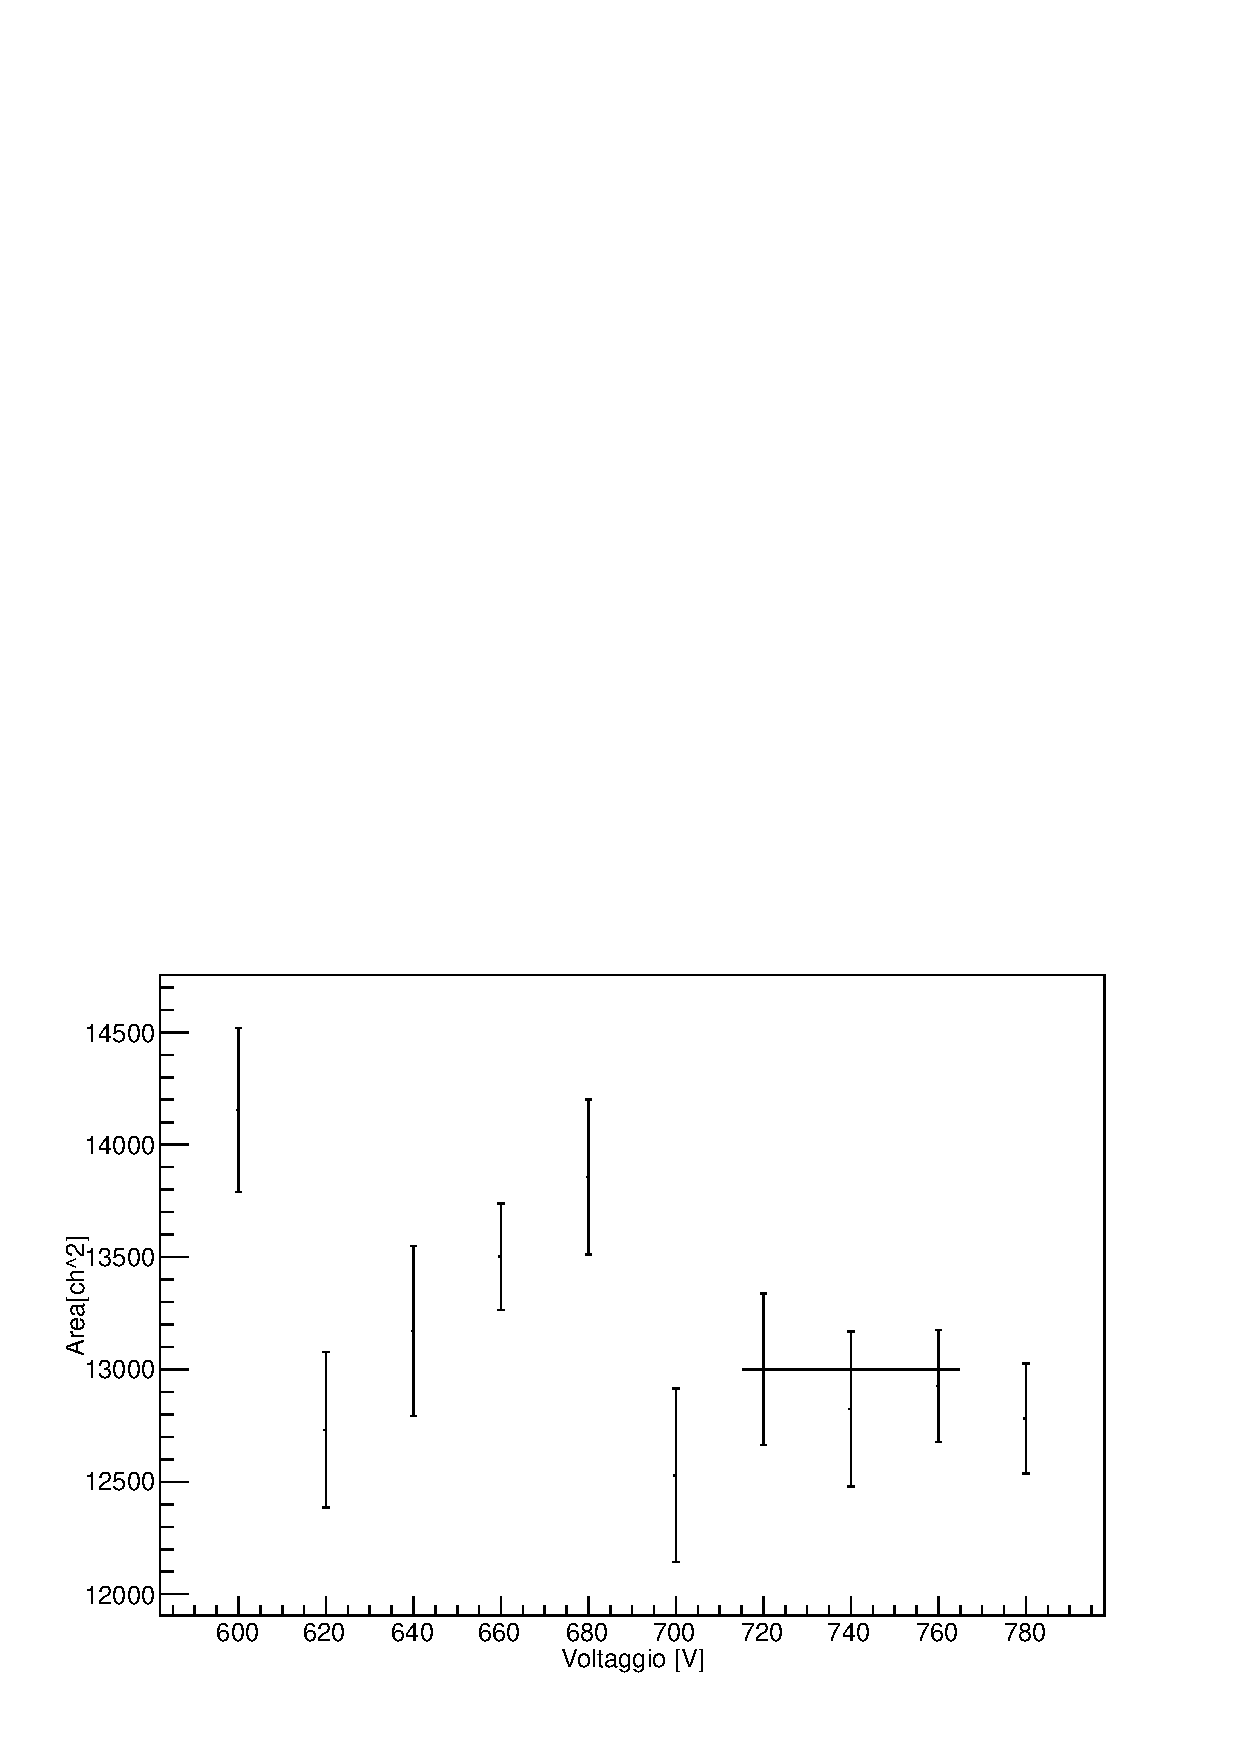
\includegraphics[width=13cm]{plateauNaI.pdf}
\caption{Dati e grafico plateau scintillatore NaI}
\end{figure}
   
\newpage
 \item $\prescript{}{}{CeBr}_{3}^{}$
   
    Il voltaggio scelto è 740V.
    \vspace{1cm}
     \begin{center}
         \begin{tabular}{cccc}
          \hline
          $\Delta$V(V) & Picco(Ch) & $\sigma_{picco}$(Ch) & Area\\
          \hline\hline
          640 &1046 & 54 & 13874$\pm$535 \\
          660& 1039 & 53 & 13680$\pm$304 \\
          680& 1019 & 52 & 138896$\pm$312 \\
         700& 1025 & 53 & 13822$\pm$360 \\
            720& 1016 & 52 & 13743$\pm$384 \\
           740& 1014 & 51 & 13782$\pm$400 \\
          760& 1013 & 50 & 12996$\pm$398 \\
           780& 1009 & 52 & 13798$\pm$436 \\
           800 & 1006 & 52 &13935 $\pm$337\\
         \hline 
          \end{tabular}
    \end{center}
    
\begin{figure}[htp]
\centering
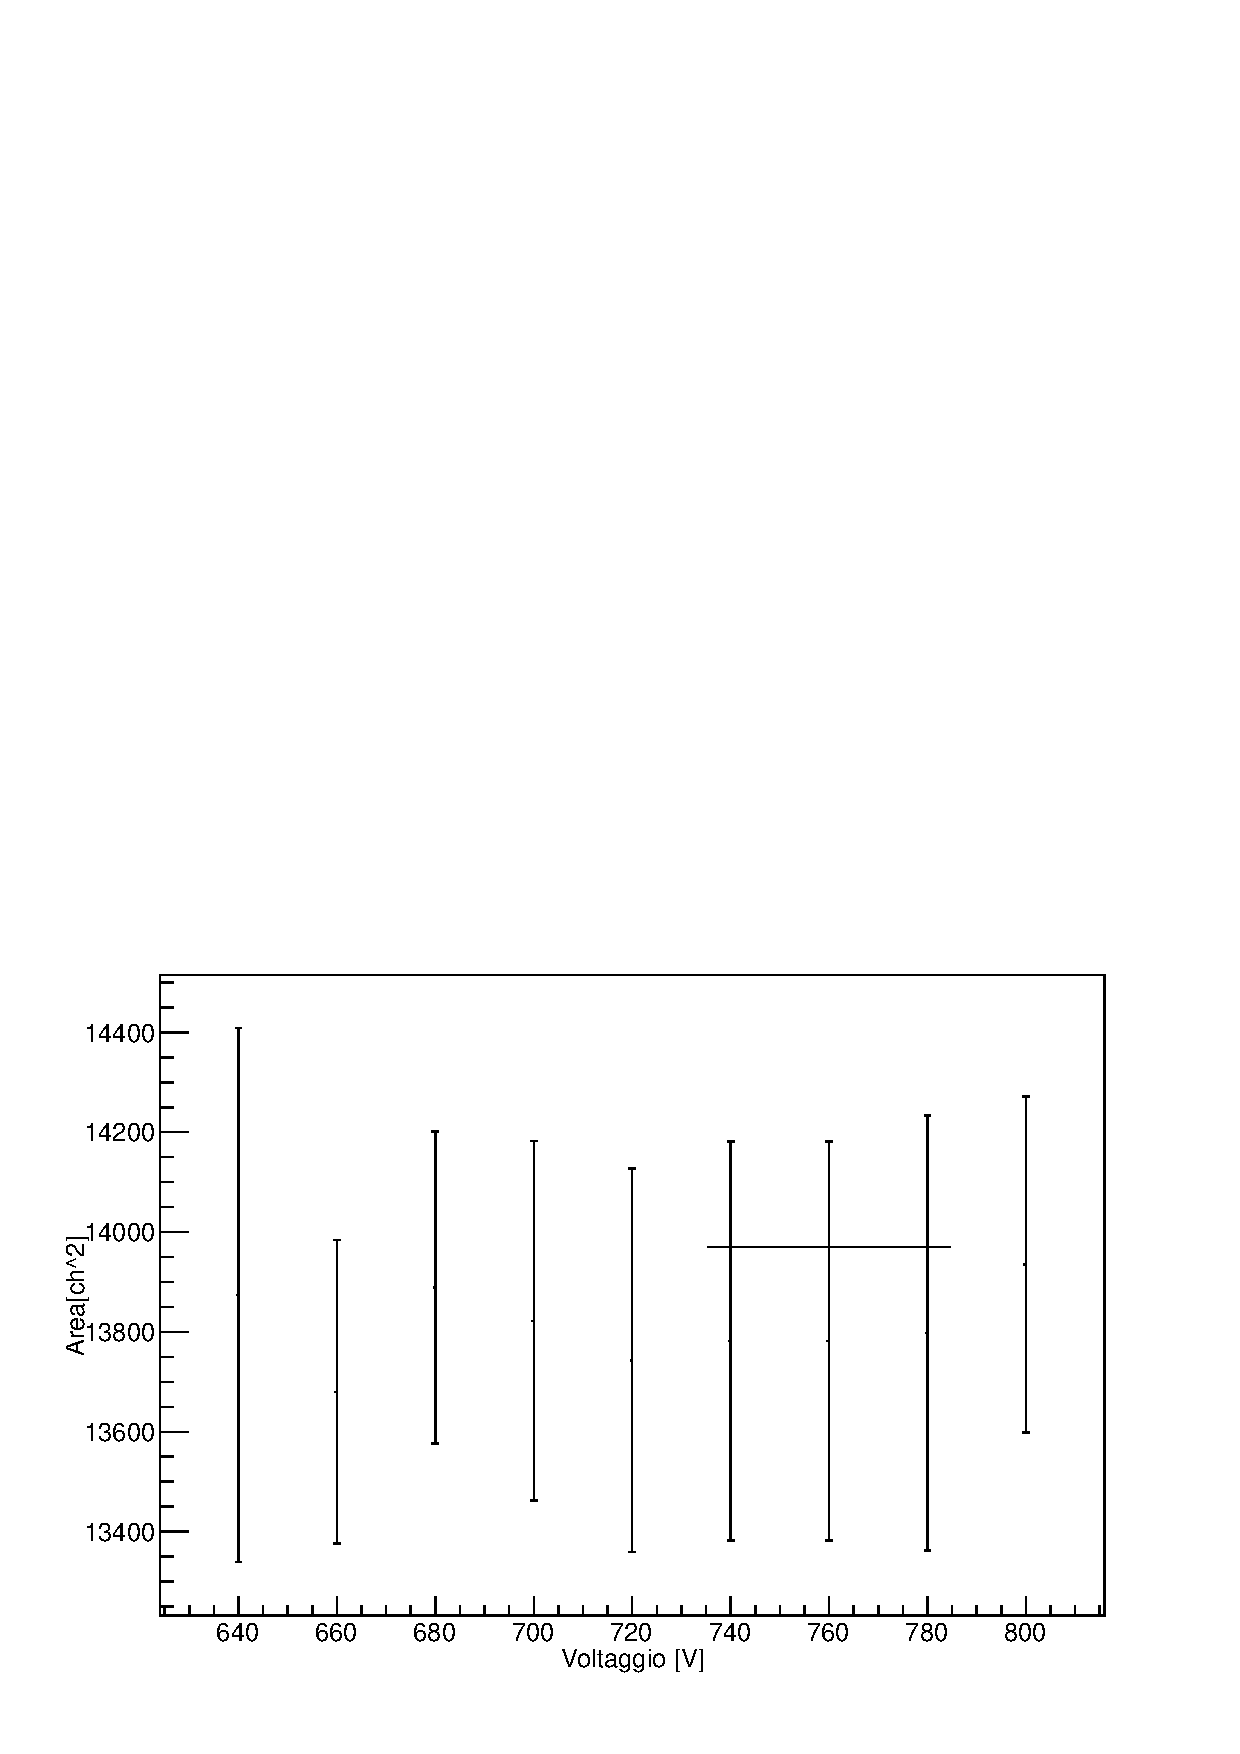
\includegraphics[width=13cm]{plateauCeBr3.pdf}
\caption{Dati e grafico plateau scintillatore $\prescript{}{}{CeBr}_{3}^{}$}
\end{figure}

 
   
   
    
\end{itemize}  

\newpage
\section{Shaping-time}
Il segnale in entrata all'amplificatore ha nella sua ampiezza (o nel suo integrale) l'informazione sull'energia depositata. In una situazione ideale, il tempo di formazione dell'amplificatore deve essere maggiore del tempo di salita del segnale. Per avere una soluzione ottimale, si fissa lo shaping-time (tempo di formazione del segnale) scegliendo il rapporto più piccolo tra FWHM e il valor medio della gaussiana risultanti dal fit. Il tempo di misura è 300s live time.



\begin{itemize}
    \item NaI: per questo rivelatore abbiamo a disposizione solo due shaping-time, 2$\mu$s e 0,5$\mu$s.

\vspace{3mm}   
    \begin{center}
   \begin{tabular}{cc}
    \hline
    Shaping-Time($\mu$s)& $\frac{FWHM}{mean}$\\
    \hline\hline
    0,5& 0,0446\\
    2& 0,0477\\
    \hline
    \end{tabular}
   \end{center}
    
    Per questo scintillatore abbiamo scelto uno shaping-time di 0,5$\mu$s.
    
 \vspace{3mm}     
    \item $\prescript{}{}{CeBr}_{3}^{}$: per questo rivelatore è possibile ottenere combinazioni differenti di tempi di integrazione e differenziazione del segnale. 
 
\vspace{3mm}  
    \begin{center}
    \centering
    \begin{tabular}{ccc}
    \hline
    Intervallo integrazione($\mu$s)& Intervallo derivazione($\mu$s)& $\frac{FWHM}{mean}$\\
    \hline\hline
    0,5& 0,5& 0,0218\\
    0,5& 1,0& 0,0198\\
    0,5& 1,5& 0,0191\\
    0,5& 2,0& 0,0172\\
    1,0& 0,5& 0,0202\\
    1,0& 1,0& 0,0203\\
    1,0& 1,5& 0,0187\\
    1,0& 2,0& 0,0189\\
    1,5& 0,5& 0,0226\\
    1,5& 1,0& 0,0192\\
    1,5& 1,5& 0,0191\\
    1,5& 2,0& 0,0176\\
    2,0& 0,5& 0,0200\\
    2,0& 1,0& 0,0215\\
    2,0& 1,5& 0,0182\\
    2,0& 2,0& 0,0171\\
    
    \hline
    \end{tabular}
    \end{center}
    
    Per questo rivelatore abbiamo scelto una combinazione di 1,5$\mu$s di integrazione e 2$\mu$s di differenziazione.
    

\end{itemize}

\vspace{3cm}
\section{Calibrazione in energia}
Questa operazione permette di stabilire una relazione tra il canale dell'istogramma in cui viene contato un segnale in input e l'energia del fotone $\gamma$ osservato. Sono  state utilizzate sorgenti differenti di cui è nota l'energia dei fotoni emessi: è stato quindi studiato il variare del valor medio del canale della gaussiana osservata in funzione dell'energia del fotone tabulata. I dati sono stati analizzati con \textit{Root} ed è stato poi ottenuto un fit lineare.

\vspace{2cm}
\begin{center}
    \centering
    \begin{tabular}{cccc}
    \hline
    Elemento& $Energia_{\gamma}$(keV)& Picco (Ch) &  $\sigma_{picco}$(Ch)\\
    \hline\hline
    $\prescript{241}{}{Am}_{}^{}$ & 59,54 & 607 & 36 \\
    Pb & 72,87 & 740 & 40 \\
    $\prescript{133}{}{Ba}_{}^{}$ & 80,99 & 808 & 49\\
    $\prescript{133}{}{Ba}_{}^{}$ & 276,40 & 2949 & 60 \\
    $\prescript{133}{}{Ba}_{}^{}$ & 302,85 & 3243 & 73 \\
    $\prescript{133}{}{Ba}_{}^{}$ & 356,01 & 3834 & 82 \\
    $\prescript{22}{}{Na}_{}^{}$ & 511,00 & 5799 & 113 \\
    $\prescript{137}{}{Cs}_{}^{}$ & 661,66 & 7241 & 133 \\
    
    \hline
    \end{tabular}
    \end{center}
\begin{figure}[htp]
\centering
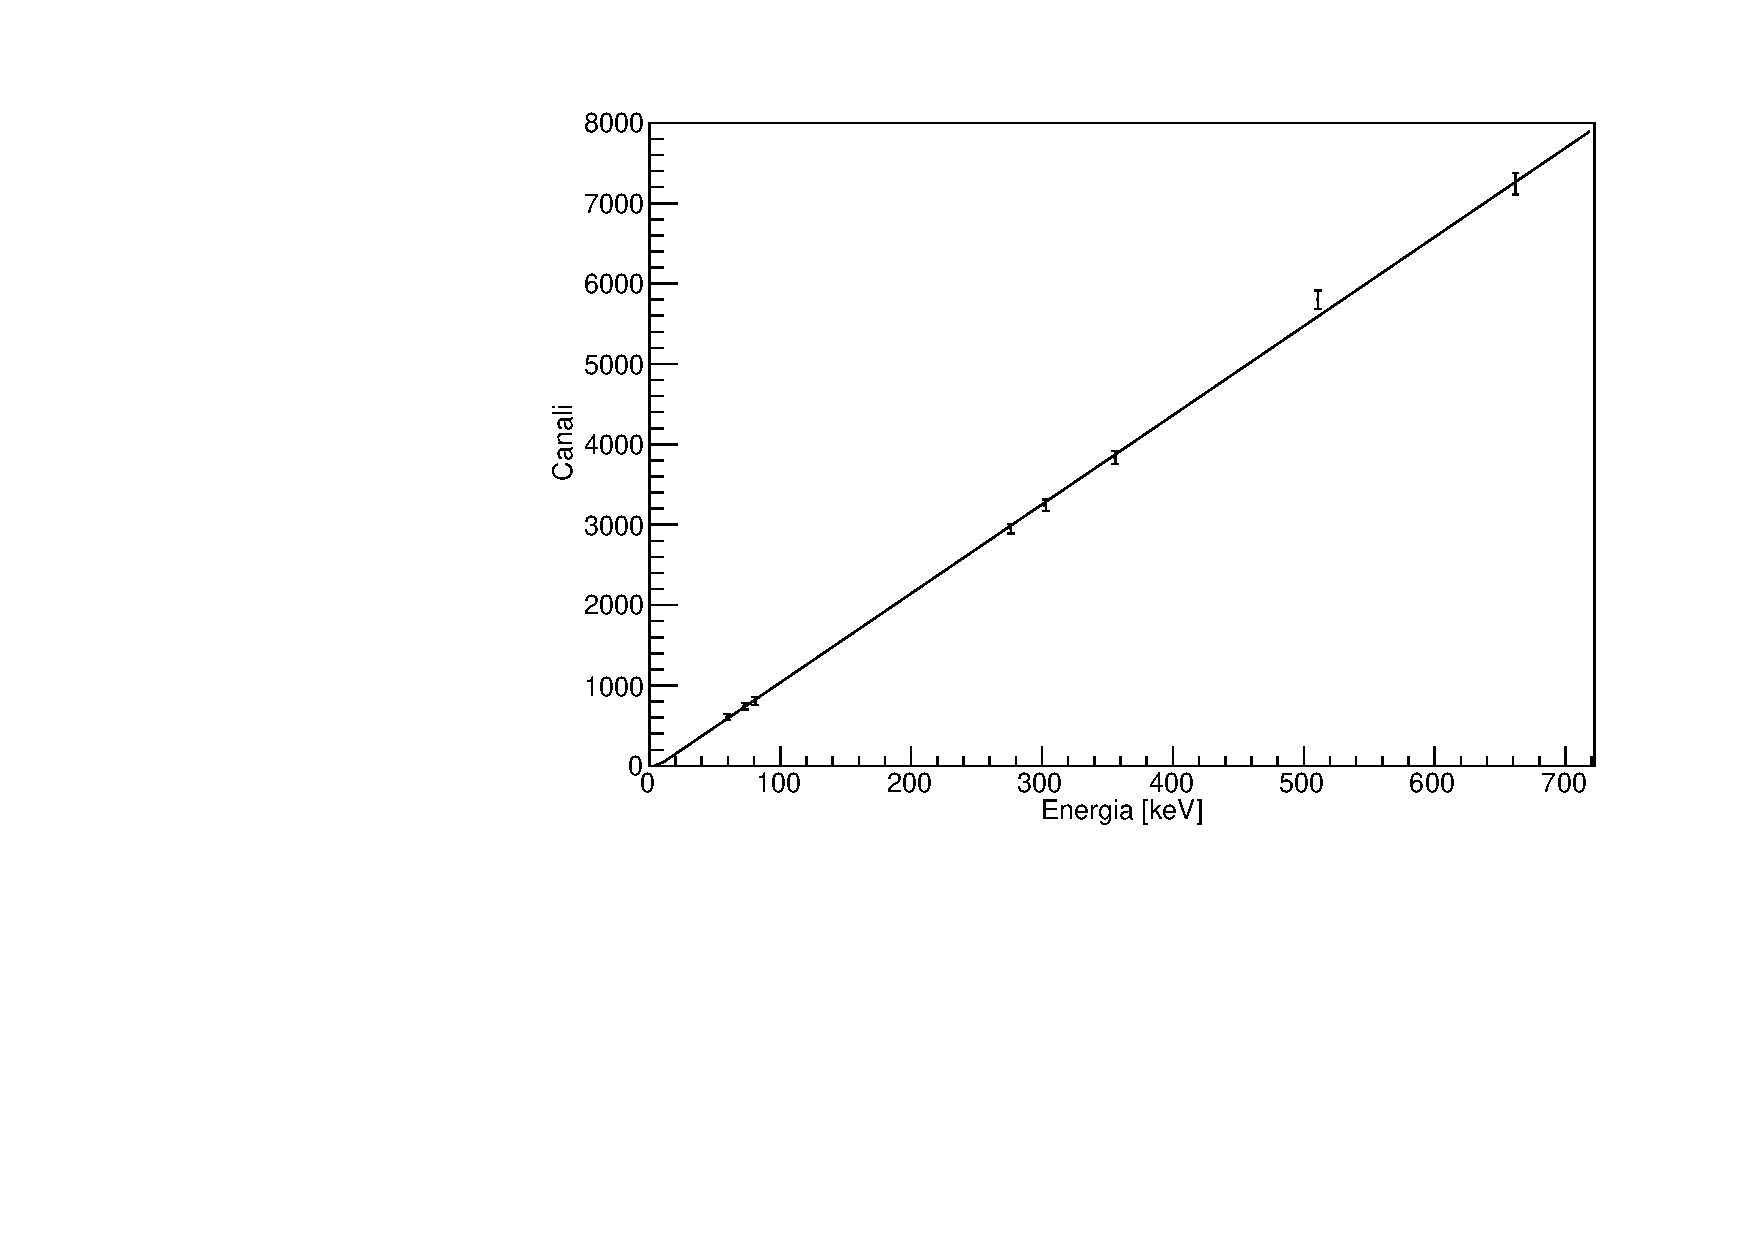
\includegraphics[width=11cm]{fit_retta_calibrazioneEnergetica.pdf}
\caption{Grafico della retta di calibrazione energetica}
\end{figure}

\vspace{10cm}
La retta di calibrazione ottenuta è: $$N_{Ch}=E_{\gamma}(11,09\pm0,14)-(72,91\pm29,05)$$ Il $\chi^2$ ridotto risulta pari a 0,69: si ha una buona compatibilità tra i dati e il fit ottenuto.

\newpage
\section{Fondo ambientale}
La misura del fondo ambientale è stata effettuata per una settimana operando senza sorgente ad un angolo $\theta$ di $0^{\circ}$. In questo modo è stato possibile ottenere lo spettro di fondo dovuto principalmente all'emissione di fotoni da parte delle mattonelle di piombo utilizzate per schermare l'intero apparato. Riportiamo di seguito l'istogramma ottenuto.

\begin{figure}[htp]
\centering
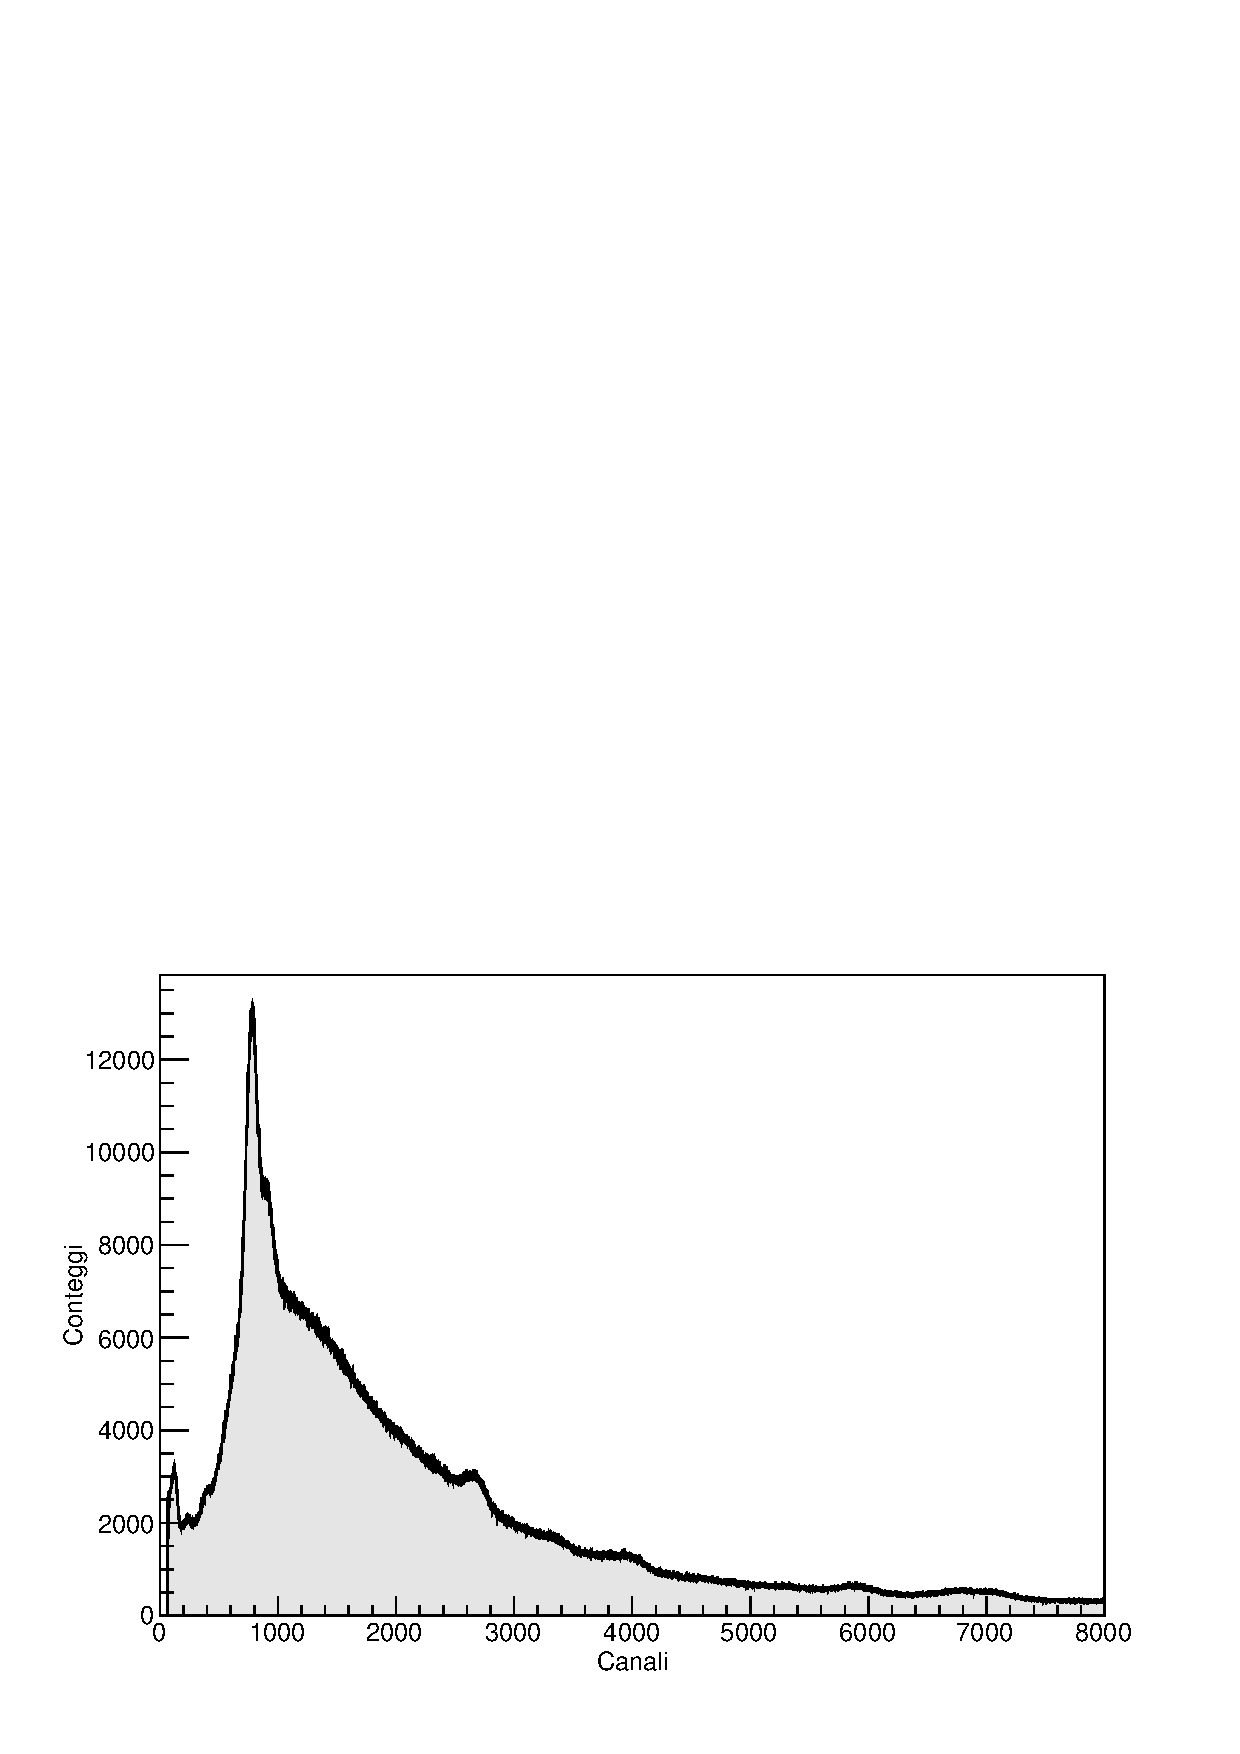
\includegraphics[width=11cm]{fondo2.pdf}
\caption{Fondo ambientale rilevato (tempo di misura: 7 giorni)}
\end{figure}



\chapter{Studio dell'efficienza}

Usando la tecnica delle misure in coincidenza è possibile studiare le efficienze dei due rivelatori. Mettere in coincidenza i due rivelatori A e B significa selezionare tra tutti i fotoni rilevati dal primo solo quelli derivanti da annichilazione elettrone-positrone, i quali hanno quindi un corrispettivo fotone $\gamma$ rilevato dal secondo scintillatore. In questa esperienza, il rilevatore NaI funge da trigger. Analizzando i segnali con l'oscilloscopio, si va a studiare il rilevatore A facendo un trigger su se stesso: si collega il rilevatore al modulo TISCA, così da avere il segnale osservato come input. In uscita si avranno due cavi output: il primo, convertito in segnale logico grazie alla funzione SCA, permette di ottenere una funzione quadra, mentre il secondo risulta essere il segnale amplificato. Il segnale logico viene generato solamente se il segnale amplificato cade all'interno di una finestra energetica [E, E+$\Delta$E] (gate) che viene impostata manualmente in modo da racchiudere l'intero fotopicco da 511keV. Per avere il segnale amplificato esattamente all'interno del segnale logico, è stato necessario ritardare il segnale di 3.30$\mu$s. Dopo aver studiato NaI triggerato su se stesso, si è proceduto a mettere in coincidenza i due rivelatori: il rilevatore A definisce il segnale logico mentre il rilevatore B fornisce quello amplificato. Il segnale non aveva bisogno di alcun ritardo. Il segnale in uscita, tramite il modulo ADC, genera un segnale rilevato da Maestro solamente se si trova all'interno del gate energetico fissato. Successivamente sono state prese misure anche senza coincidenza. Questo ha permesso lo studio dell'efficienza intrinseca dei due strumenti. Definendo infatti con 

\begin{itemize}
    \item n(A) il numero di fotoni da 511keV rilevati da A
    \item n(B) il numero di fotoni da 511keV rilevati da B
    \item n(A:B) il numero di fotoni rilevati da B in coincidenza con A (A funge da trigger)
    \item n(B:A) il numero di fotoni rilevati da A in coincidenza con B (B funge da trigger)
\end{itemize}
Valgono allora le seguenti relazioni:

\[ n(A)=2S\Delta t  \cdot e(A,E) \cdot \frac{\Delta \Omega}{4 \pi} \]
\[ n(B)=2S\Delta t  \cdot e(B,E) \cdot \frac{\Delta \Omega}{4 \pi} \]
\[ n(A:B)=n(B:A)=2S\Delta t  \cdot e(A,E) \cdot e(B,E)\frac{\Delta \Omega}{4 \pi} \]
dove S rappresenta l'attività della sorgente in Bq, $\Delta$t il tempo di misura, e(A,E) e e(B,E) le efficienze intrinseche dei due rivelatori, $\frac{\Delta \Omega}{4 \pi}$ l'angolo solido sotteso dai rivelatori (uguale per entrambi). Il fattore due indica che a ogni disintegrazione corrispondono due fotoni. Si ottengono quindi le efficienze intrinseche dei due rivelatori:

\[ e(A,E)=\frac{n(A:B)}{n(B)} \]

\[ e(B,E)=\frac{n(B:A)}{n(A)} \]

Le misure relative sono state effettuate individuando la distanza dalla sorgente tale per cui si ha uno stesso angolo solido sotteso dai rivelatori, facendo una proporzione tra il diametro dei rivelatori e la distanza dalla sorgente stessa. 
%%DISEGNO DISTANZA RILEVATORI-ANGOLO SOLIDO
 La scelta delle distanze tra i rivelatori e la sorgente risulta essere il compromesso tra un buon tasso di conteggio, che porterebbe ad avvicinare la sorgente allo scintillatore, e una buona precisione della misura dell'energia del fotone al variare dell'angolo di diffusione, che porterebbe alla scelta opposta. 

\begin{center}
    \centering
    \begin{tabular}{cc}
    \hline
    diametro A & 3,80$\pm$0,05cm \\
    \hline
    diametro B & 4,20$\pm$0,05cm \\
    \hline
    distanza massima & 62,0$\pm$0,1cm\\
    \hline
    \end{tabular}
    \end{center}

Le distanze tra rivelatori e sorgente tali da sottendere uno stesso angolo solido sono $l_{As}$=24,6cm e $l_{Bs}$=37,4cm.

Una volta individuata la posizione ideale si avvicina la sorgente al rivelatore di cui si vuole misurare l’efficienza, in modo che il cono di angolo solido corrispondente ai fotoni che hanno interagito nell’altro rivelatore investa solo la porzione centrale del rivelatore stesso. In questo modo si rende massima la probabilità di totale contenimento di un’eventuale interazione.
\begin{itemize}
    \item Rivelatore A 
    \begin{center}
    \centering
    \begin{tabular}{ccc}
    \hline
    & Rivelatore A& Rivelatore B\\
    \hline\hline
    segnale& analogico& logico\\
    gate& - & $E_{0}$=3,30  $\Delta$E=1,30\\
    guadagno& INSERIRE& INSERIRE\\
    \hline
    \end{tabular}
    \end{center}
    
    \vspace{0.3cm}
   \begin{center}
    \centering
    \begin{tabular}{ccccc}
    \hline
    $l_{As}$(cm)& $l_{Bs}$(cm)& n(B) &  n(A:B)& e(A)\\
    \hline\hline
    23& 39& 9747$\pm$690& 2293$\pm$271 & 0,24$\pm$0,03\\
    21& 41& 8278$\pm$903& 1493$\pm$272& 0,18$\pm$0,04\\
    19& 43& 8449$\pm$828& 1668$\pm$237& 0,20$\pm$0,03\\
    \hline
    \end{tabular}
    \end{center}
Il valore ottenuto tramite media pesata è e(A)=(20,1$\pm$2,0)$\%$.    
    
    \vspace{0.3cm}
    
    \item Rivelatore B
      \begin{center}
    \centering
    \begin{tabular}{ccc}
    \hline
    & Rivelatore A& Rivelatore B\\
    \hline\hline
    segnale& logico& analogico\\
    gate& $E_{0}$=3,40  $\Delta$E=1,70& -\\
    guadagno& INSERIRE& INSERIRE\\
    \hline
    \end{tabular}
    \end{center}
  \vspace{0.3cm}   
   \begin{center}
    \centering
    \begin{tabular}{ccccc}
    \hline
    $l_{As}$(cm)& $l_{Bs}$(cm)& n(A) &  n(B:A)& e(B)\\
    \hline\hline
    25& 37& 9819$\pm$442& 2241$\pm$47 & 0,23$\pm$0,01\\
    27& 35& 10439$\pm$547& 2223$\pm$130& 0,20$\pm$0,02\\
    29& 33& 12083$\pm$356& 2126$\pm$140& 0,18$\pm$0,13\\
    \hline
    \end{tabular}
    \end{center}
Il valore ottenuto tramite media pesata è e(B)=(20,5$\pm$0,8)$\%$.
\end{itemize}

\chapter{Disposizione dell'apparato}
\section{Verifica della calibrazione del sistema}
Prima di procedere con le misure, è stata verificata la corretta calibrazione dei dispositivi perchè, per motivi tecnici, è stato necessario staccare la corrente all'intero impianto. Osservando il segnale del fotone rilevato e il segnale logico del trigger, abbiamo deciso di ritardare il segnale in ingresso di 1$\mu$s perchè non si aveva più una sovrapposizione tra i due impulsi. Questo ha portato alla necessità di fare una nuova calibrazione in energia per avere una corretta relazione tra bin rilevato e energia del fotone. Riportiamo di seguito le misure ottenute.
\vspace{3mm}  

\begin{center}
    \centering
    \begin{tabular}{cccc}
    \hline
    Elemento& $Energia_{\gamma}$(keV)& Picco (Ch) &  $\sigma_{picco}$(Ch)\\
    \hline\hline
    $\prescript{241}{}{Am}_{}^{}$ & 59,54 & 579 & 38 \\
    Pb & 72,87 & 748 & 44 \\
    $\prescript{133}{}{Ba}_{}^{}$ & 276,40 & 2999 & 92 \\
    $\prescript{133}{}{Ba}_{}^{}$ & 302,85 & 3288 & 70 \\
    $\prescript{133}{}{Ba}_{}^{}$ & 356,01 & 3885 & 91 \\
    $\prescript{22}{}{Na}_{}^{}$ & 511,00 & 5679 & 109 \\
    $\prescript{137}{}{Cs}_{}^{}$ & 661,66 & 7412 & 129 \\
    
    \hline
    \end{tabular}
    \end{center}
 La nuova retta di calibrazione è: 
 $$N_{Ch}=E_{\gamma}(11,24\pm0,15)-(87,91\pm33,92)$$ Il $\chi^2$ ridotto risulta pari a 0,14.
 
 \vspace{3mm}
 
 \begin{figure}[htp]
\centering
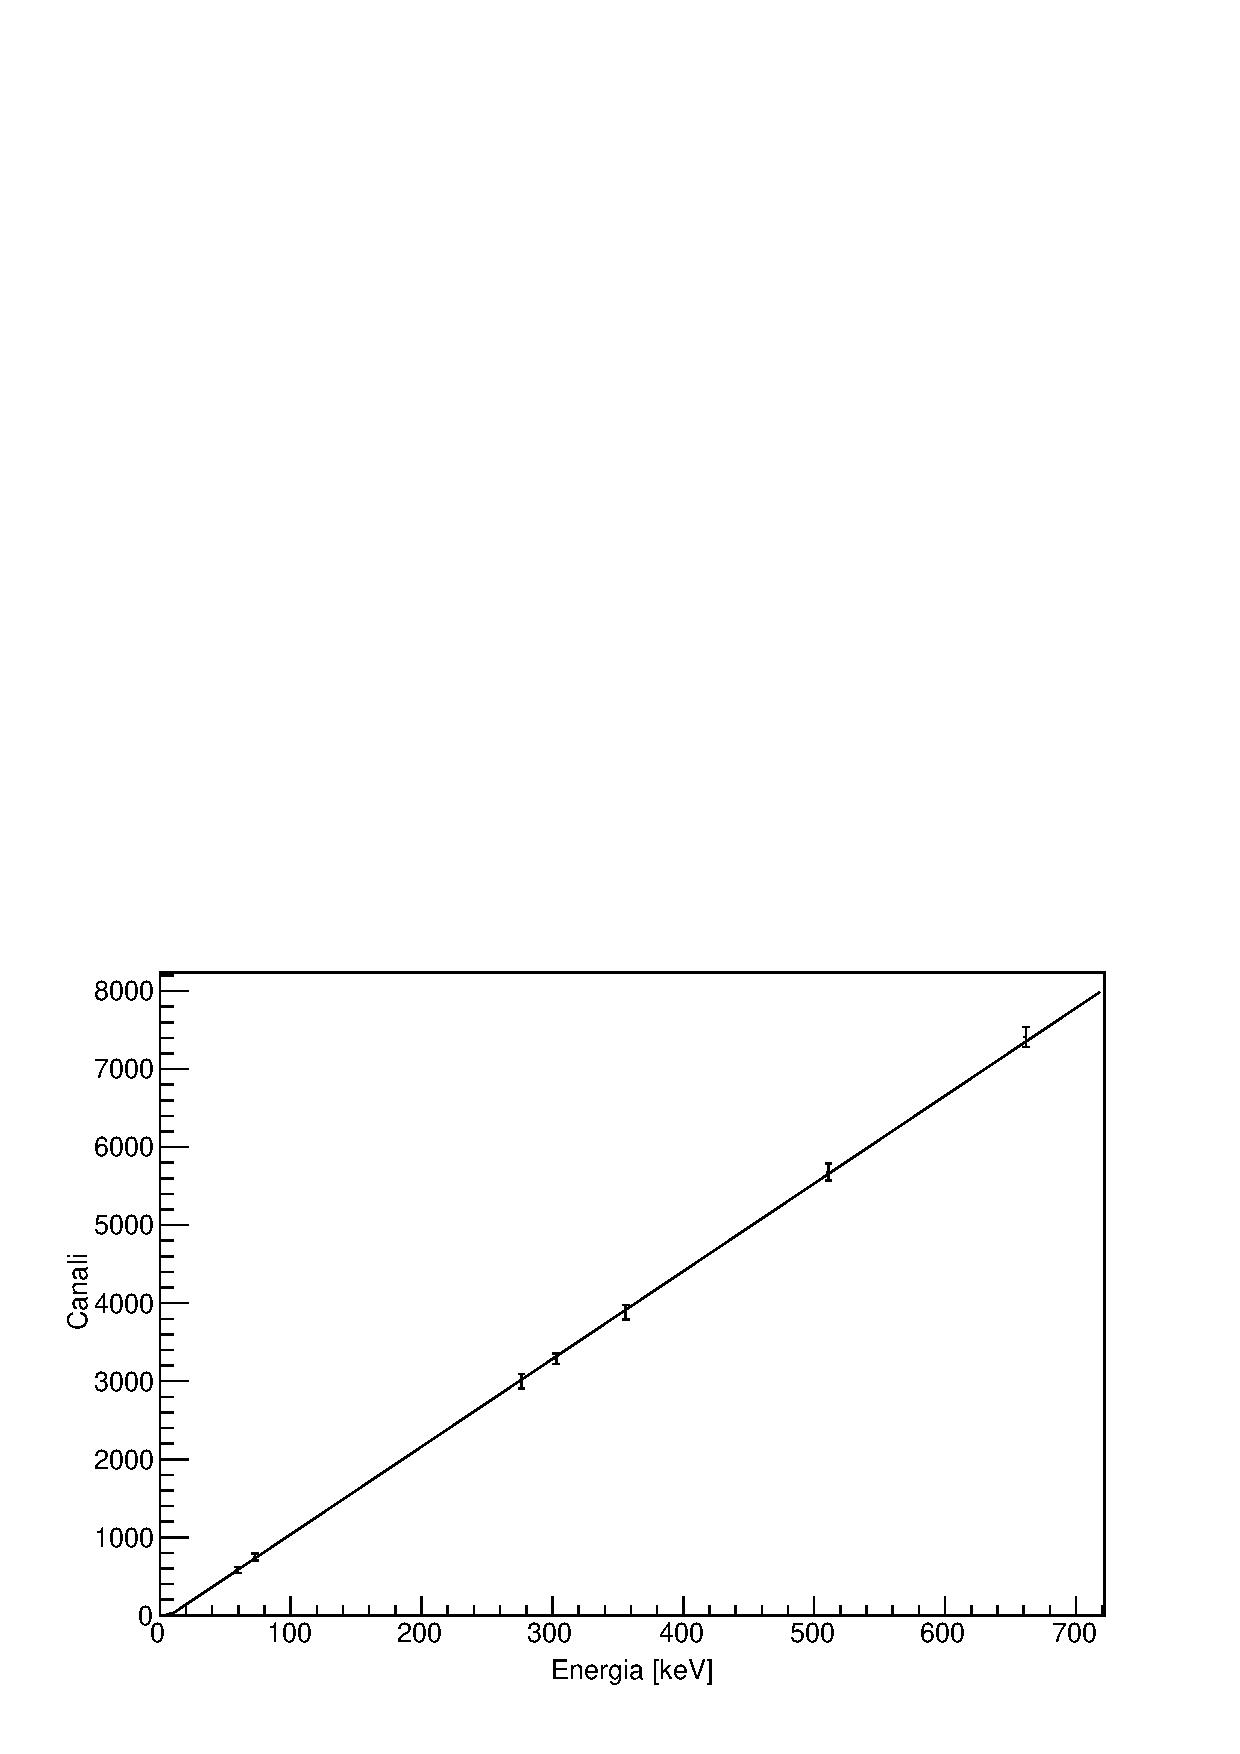
\includegraphics[width=11cm]{regressione.pdf}
\caption{Grafico della retta di calibrazione energetica}
\end{figure}
 
  \vspace{3mm}
  \vspace{3mm}
  \vspace{3mm}
Dato che il segnale risultava particolarmente lungo rispetto al segnale logico, è stata valutata l'ipotesi di ricalibrare il sistema variando i valori di integrazione e differenziazione del segnale del $CeBr_{3}$. Abbiamo quindi preso misure sia in coincidenza che non (sempre utilizzando NaI come trigger) con i valori di integrazione e differenziazione di 1,5-2 (come scelto in precedenza) e di 1-1 (in cui si ha un segnale più alto e stretto). Abbiamo quindi misurato le aree dei fotopicchi da 511keV. 

\vspace{3mm}  

 \begin{center}
    \centering
    \begin{tabular}{cccc}
    \hline
    Misura& Integrazione& Differenziazione& Area fotopicco\\
    \hline\hline
    Coincidenza & 1,5 & 2,0& 2235$\pm$47\\
    Coincidenza & 1,0& 1,0& 2284$\pm$47\\
    Non coincidenza & 1,5 & 2,0& 9521$\pm$488\\
    Non coincidenza& 1,0& 1,0& 9602$\pm$426\\
    
    \hline
    \end{tabular}
    \end{center}
    
    
Le aree ottenute risultano praticamente uguali: questo implica che non vengono persi eventi con le impostazioni 1,5-2 nonostante la coda del segnale non sia pienamente contenuta nel segnale logico. 

\section{Disposizione del banco}
In questa fase dell'esperimento abbiamo scelto in che modo disporre la strumentazione. Come bersaglio tramite cui deviare i fotoni emessi si utilizza una targhetta di piombo dello spessore di 2,4$\pm$0,5mm. 

\begin{figure}[htp]
\centering
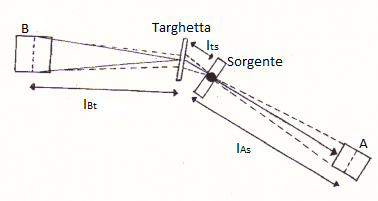
\includegraphics[width=11cm]{apparato.png}
\caption{Disposizione del banco}
\end{figure}
La distanza ottimale tra sorgente, targhetta e rivelatori risulta essere il compromesso tra la necessità di avere sorgente e rivelatore vicini per avere un numero significativo di eventi e distanze maggiori tra gli stessi per avere una buona precisione nella misura dell'energia ad un determinato angolo. Abbiamo analizzato un fotopicco a 511keV facendo un fit con root e abbiamo ottenuto una risoluzione $\frac{\Delta E}{E}$ del 4$\%$.
Dalla relazione (1.1) si ottiene l'equazione differenziale
\vspace{0.5cm}
\begin{align*}
d\theta&=\frac{2-cos(\theta)}{sen\theta}\frac{dE'}{E'}\\
\end{align*}
che ammette un minimo per $\theta$=$\frac{\pi}{3}$. Al minimo, con la risoluzione trovata prima, si ottiene una distanza tra rivelatore B e targhetta $l_{Bt}$=54cm. Per avere un maggior numero di eventi rilevati a parità di tempo, abbiamo scelto di ridurre questa distanza. A livello teorico, questa distanza risulta essere data dalla relazione
\vspace{0.5cm}
\begin{align*}
l_{Bt}\tan\frac{\theta}{2}&=\frac{d_{B}}{2}\\
\end{align*}
dove $d_{B}$  è il diametro del rivelatore B. Per ottenere poi la distanza tra la sorgente e il rivelatore A si impone semplicemente un'uguaglianza tra gli angoli solidi sottesi dai due rivelatori rispetto alla sorgente. 
Per avere un numero maggiore di eventi, abbiamo fissato la distanza $l_{Bt}$=30cm e la distanza $l_{ts}$=10cm (quest'ultima può essere scelta arbitrariamente). Per avere uno stesso angolo solido sotteso dai due rilevatori considerando la sorgente puntiforme, si ottiene una distanza tra rivelatore A e sorgente di $l_{As}$=26cm. La targhetta è stata disposta lungo la bisettrice dell'angolo di diffusione, in modo che tutti i fotoni deviati di un angolo $\theta$ attraversino lo stesso spessore D.


\begin{center}
    \centering
    \begin{tabular}{cc}
    \hline\hline
    $l_{Bt}$ & 30,0$\pm$0,1cm\\
    $l_{ts}$ & 10,0$\pm$0,1cm\\
    $l_{As}$ & 26,0$\pm$0,1cm\\
    \hline\hline
    \end{tabular}
    \end{center}
    
\chapter{Esperimento}
\section{Parte teorica: sezione d'urto}
La sezione d'urto differenziale relativa all'effetto Compton è data da
\begin{equation}
\frac{d\sigma}{d\Omega}=\frac{r^2_{e}}{2}\Biggl(\frac{E'}{E}\Biggl)^2\Biggl(\frac{E}{E'}+\frac{E'}{E}-sin^2\theta\Biggl)
\end{equation}
dove E è l'energia del fotone incidente, E' quella del fotone diffuso e $r_{e}$=2,8179$\cdot10^{-13}$ è il raggio classico dell'elettrone. \newline Dobbiamo ora trovare un'espressione che ci consenta, attraverso i dati raccolti, di calcolare la sezione d'urto differenziale. Noi possiamo solo misurare il numero di fotoni contati dal rivelatore nella zona del picco per il fotone scatterato, ossia l'area della gaussiana fittata. 
Sia ${dn}$ il numero di fotoni interagenti in uno spessore ${dx}$ della targhetta immerso a profondità ${x}$ nel bersaglio e poi contati dal rivelatore B; si ottiene

\begin{equation}
dn=nN\frac{d\sigma}{d\Omega_B}d\Omega_Be(B,E')f(x,D,\theta)dx
\end{equation}

dove $n=n(A)=2Se(A,E)t\frac{\Delta\Omega_A}{4\pi}$ è il numero di fotoni incidenti sulla targhetta corrispondenti ai fotoni con $E$=511 keV contati dal rivelatore A; $N=\rho N_a \frac{Z}{A}$ è il numero di elettroni per centimetro cubo del bersaglio (per il Pb $N$=2,707$\cdot10^{-24}$ $cm^{-3}$); $f(x,D,\theta)$ è il fattore di attenuazione per eventi di diffusione a un angolo $\theta$ che avvengono a profondità $x$ nel bersaglio. 
Riguardo al fattore di attenuazione teniamo conto della configurazione scelta per il bersaglio (lungo la bisettrice), che è la più semplice per il calcolo del fattore $f$; poniamo $D'=\frac{D}{\cos{\theta/2}}$ e calcoliamo 

\begin{equation}
f(x,D',\theta)=P(x,\lambda)P(D'-x,\lambda')
\end{equation}

dove $P(x,\lambda)=exp(-x/\lambda)$ rappresenta la probabilità che un fotone incidente arrivi a profondità $x$ nel bersaglio; invece $P(D'-x)=exp[-(D'-x)/\lambda']$ è la probabilità che un fotone diffuso riesca ad attraversare il rimanente spessore $D'-x$ di bersaglio; $\lambda$ e $\lambda'$ sono i coefficienti di attenuazione per fotoni di energia rispettivamente $E$ ed $E'$.

Possiamo ora definire il coefficiente di attenuazione Compton come

\begin{equation}
\lambda_C=\Biggl(N\frac{d\sigma}{d\Omega_B}d\Omega_B\Biggl)^{-1}
\end{equation}

ed essendo $\frac{dx}{\lambda_C}$ la probabilità di interazione dei fotoni tra $x$ e $x$+$dx$ otteniamo

\begin{equation}
dn=ne(B,E')exp\Biggl(-\frac{x}{\lambda}\Biggl)\frac{dx}{\lambda_C}exp\Biggl(-\frac{D'-x}{\lambda'}\Biggl)
\end{equation}

Integrando otteniamo il numero di fotoni contati dal rivelatore B

\begin{equation}
\Delta n=nN\frac{d\sigma}{d\Omega_B}d\Omega_{B}e(B,E')\lambda\int_{0}{D'}{exp\Biggl(-\frac{x}{\lambda}\Biggl)\frac{dx}{\lambda}exp\Biggl(-\frac{D'-x}{\lambda'}\Biggl)}
\end{equation}

Indicando ora con K

\begin{equation}
K=\int_{0}{D'}{e^{(-\frac{x}{\lambda})}\frac{dx}{\lambda}e^{(-\frac{D'-x}{\lambda'})}}=\lambda''e^{(-\frac{D'}{\lambda'})}\Biggl[1-e^{(-\frac{D'}{\lambda''})}\Biggl]
\end{equation}

dove

\begin{equation}
\lambda''=\frac{\lambda\lambda'}{\lambda-\lambda'}
\end{equation}

Otteniamo quindi la seguente espressione di cui sono note tutte le variabili per misurare la sezione d'urto differenziale:

\begin{equation}
\frac{d\sigma}{d\Omega}=\frac{\Delta n}{nNd\Omega_Be(B,E')K}
\end{equation}

\newpage
\section{Dati sperimentali}
Riportiamo gli spettri acquisiti per diversi angoli. 
Gli ultimi dati acquisiti sono stati quelli a $20^\circ$ e a $45^\circ$. A causa di uno spegnimento inatteso dell'apparato, prima di procedere con queste misure è stata verificata la calibrazione del gate energetico del trigger. Studiando lo spettro del trigger di NaI su se stesso come descritto nell'apposito paragrafo, la gaussiana rappresentante il picco a 511keV risultava decentrata rispetto alla finestra energetica impostata. Abbiamo quindi proceduto ad una nuova calibrazione, impostando i valori di gate di E=352 e $\Delta$E=140.
\vspace{1cm}

\subsection{Angolo 20$^\circ$}
I problemi riscontrati in questa misura sono stati causati dai pochi dati raccolti a causa di uno spegnimento inatteso dell'apparato. Oltre al picco cercato era visibile anche quello a 511keV, corrispondente ad un fotone non deviato. Abbiamo proceduto ad analizzare lo spettro acquisito utilizzando lo spettro relativo ad un angolo di 0$^\circ$: quest'ultimo è stato normalizzato in funzione dello spettro a 20$^\circ$ (la notevole differenza nel numero di eventi rilevati è data dalla differenza dei tempi di acquisizione del segnale). Dato che questa normalizzazione in funzione del tempo di esecuzione non era ancora sufficiente per rendere paragonabili i due spettri, è stato fatto un riscalamento manuale dello spettro a 0$^\circ$ dividendo ulteriormente per 1000. I due spettri sono quindi stati sovrapposti ed è stata fatta la differenza tra lo spettro a 20$^\circ$ e quello a 0$^\circ$. I valori che risultavano essere negativi sono stati posti a zero (un valore negativo nell'istogramma non avrebbe avuto alcun senso). Una volta completate queste fasi preliminari, abbiamo proceduto analizzando il picco osservato con il programma Root da cui abbiamo ricavato l'area della gaussiana sottesa e il canale relativo al picco.

\begin{figure}[htp]
\centering
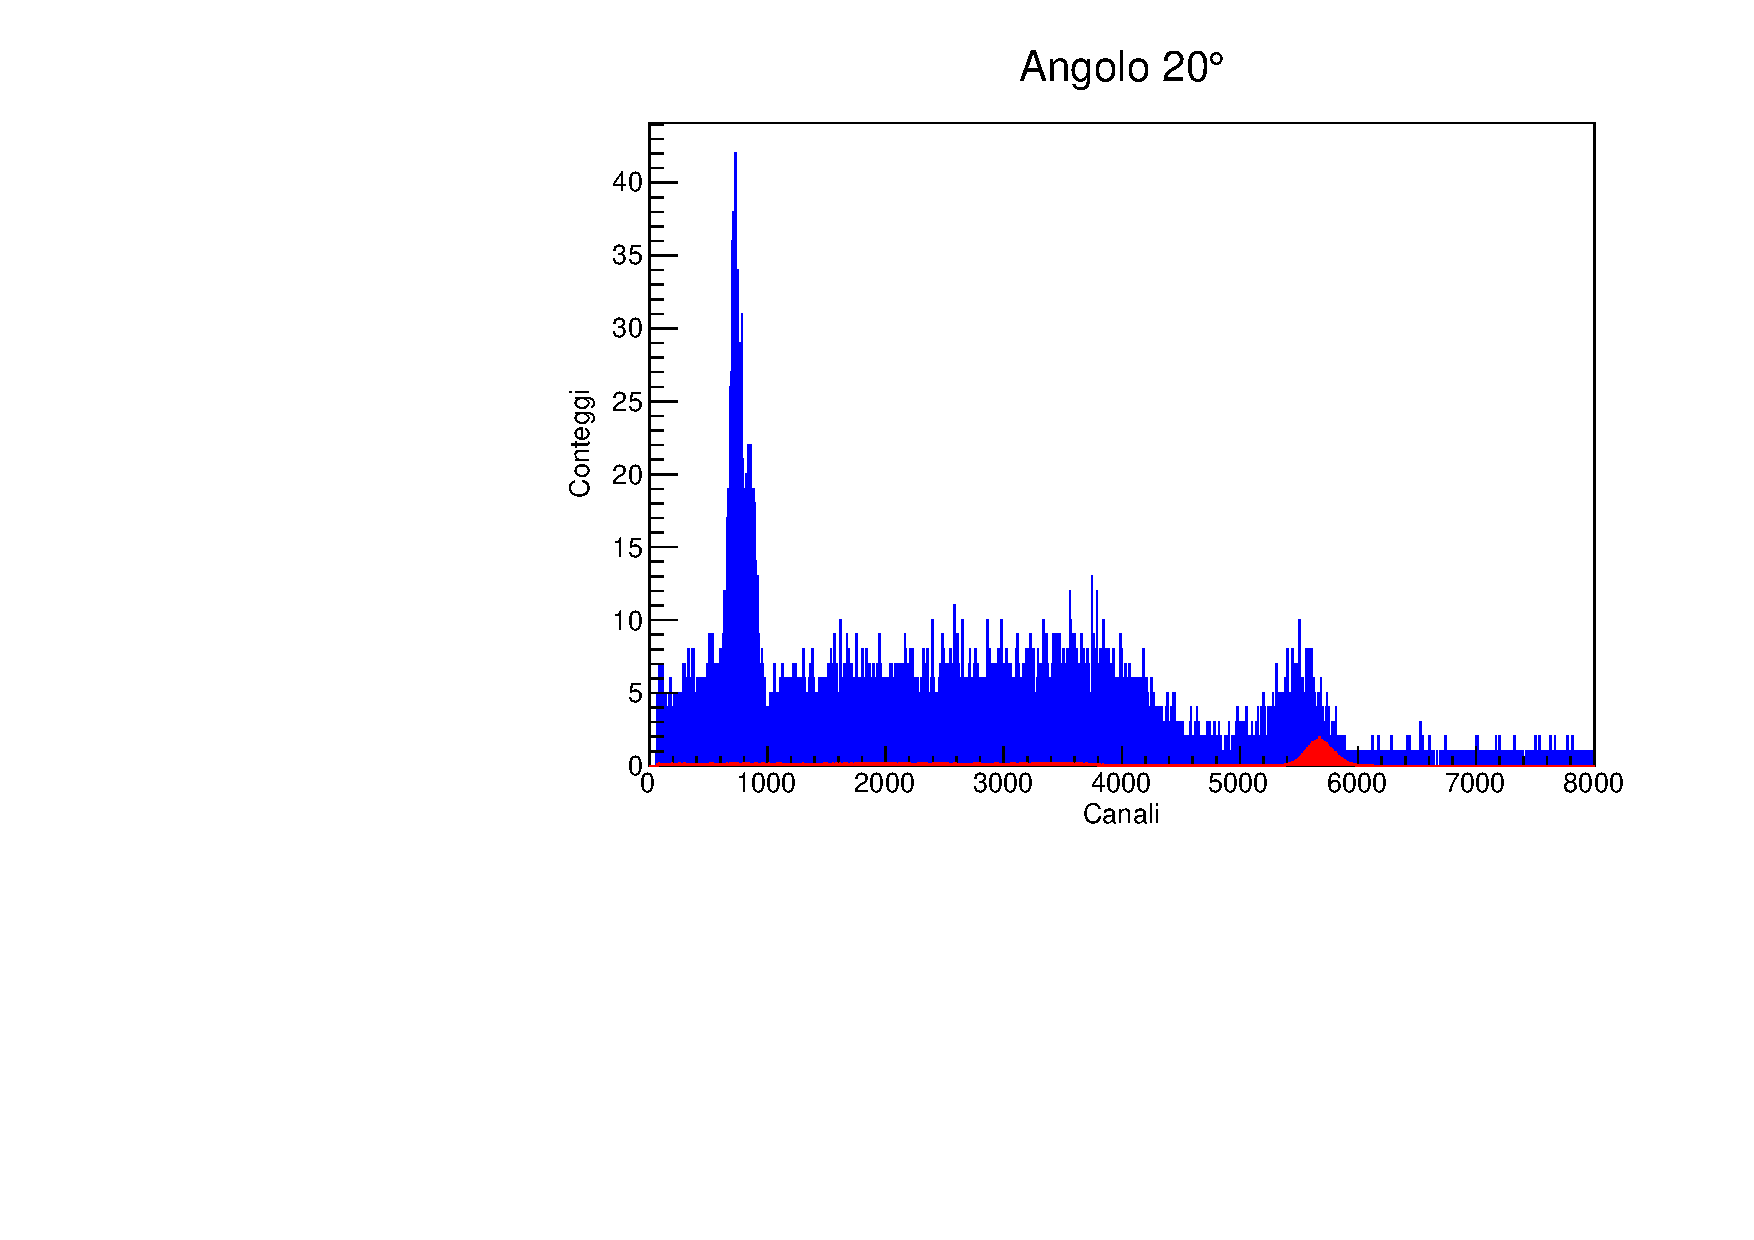
\includegraphics[width=12cm]{20originale.pdf}
\caption{Spettro rilevato a 20$^\circ$ con sovrapposizione dello spettro a 0$^\circ$ normalizzato}
\end{figure}
\begin{figure}[htp]
\centering
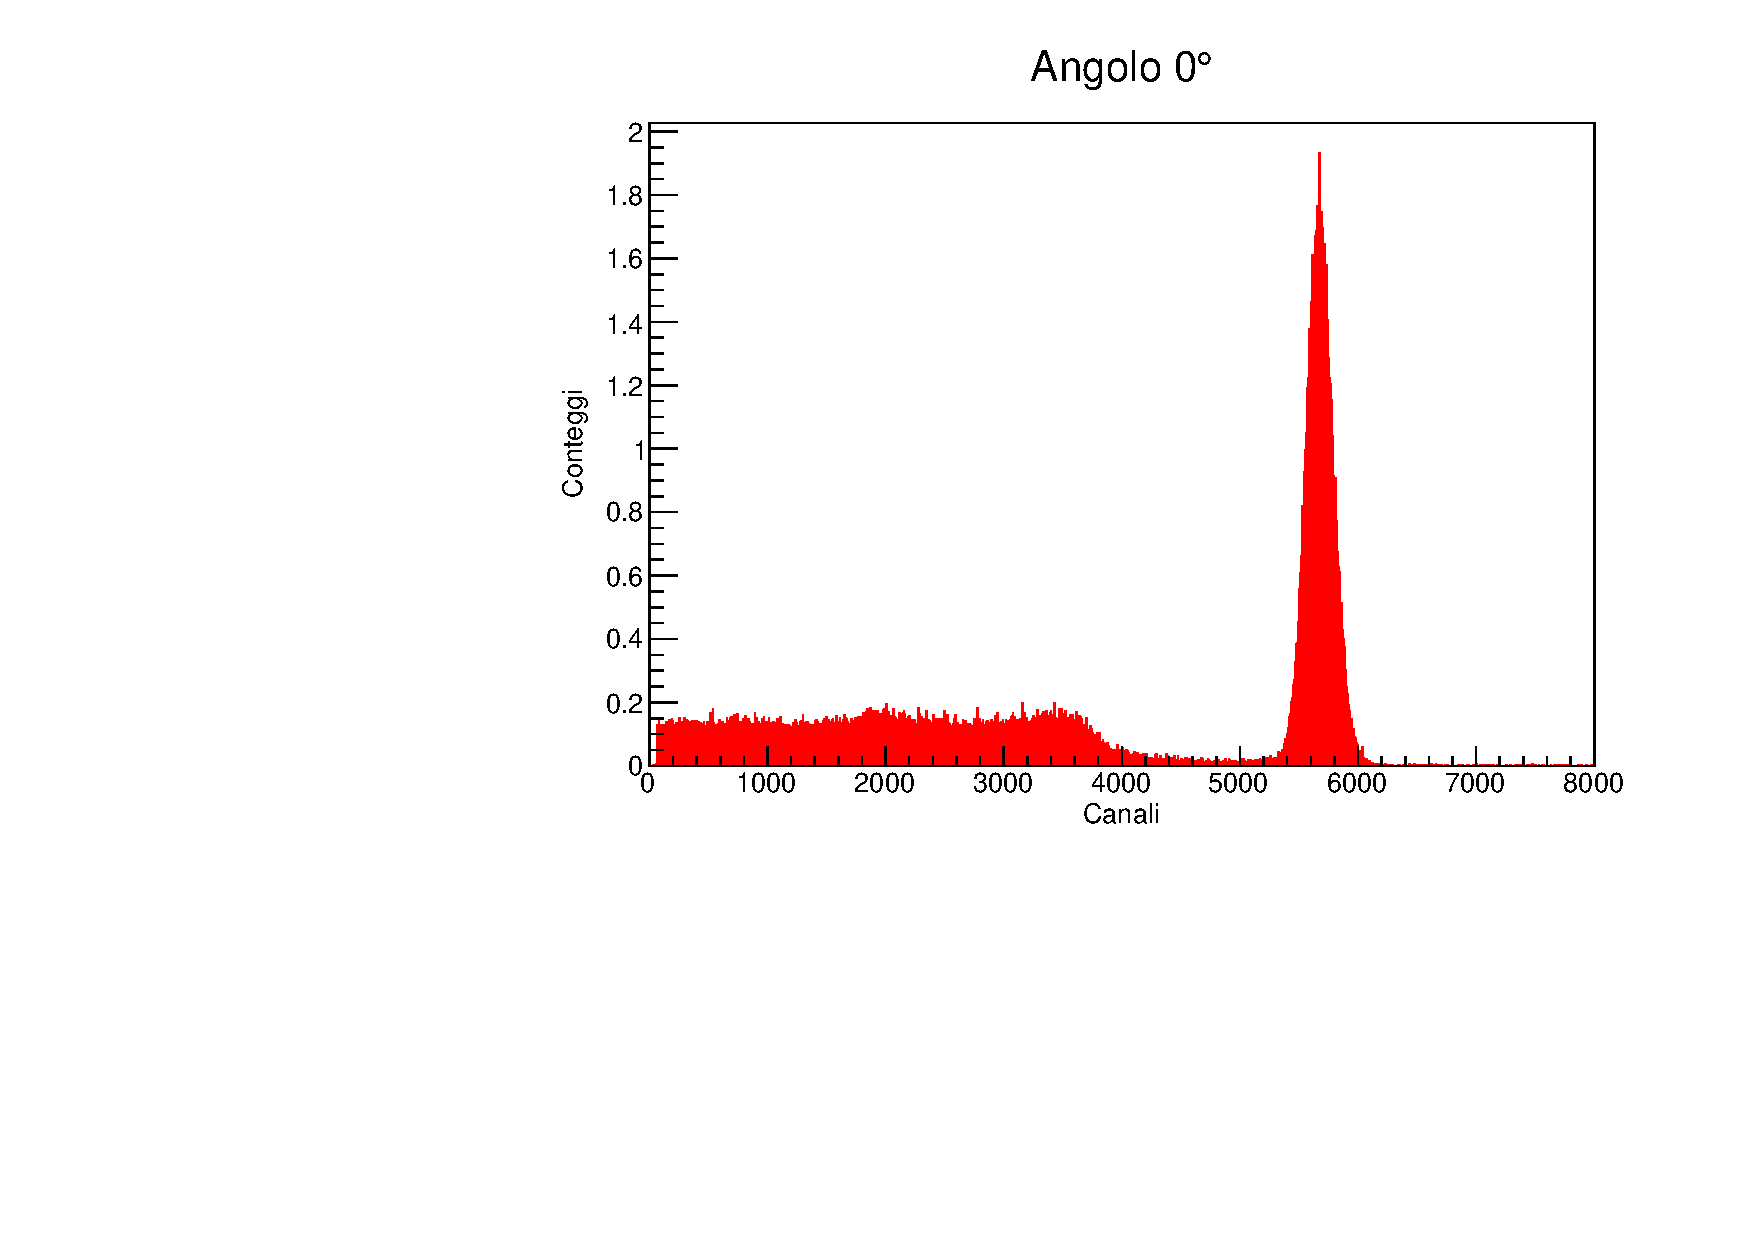
\includegraphics[width=12cm]{0originale.pdf}
\caption{Spettro rilevato a 0$^\circ$}
\end{figure}
\begin{center}
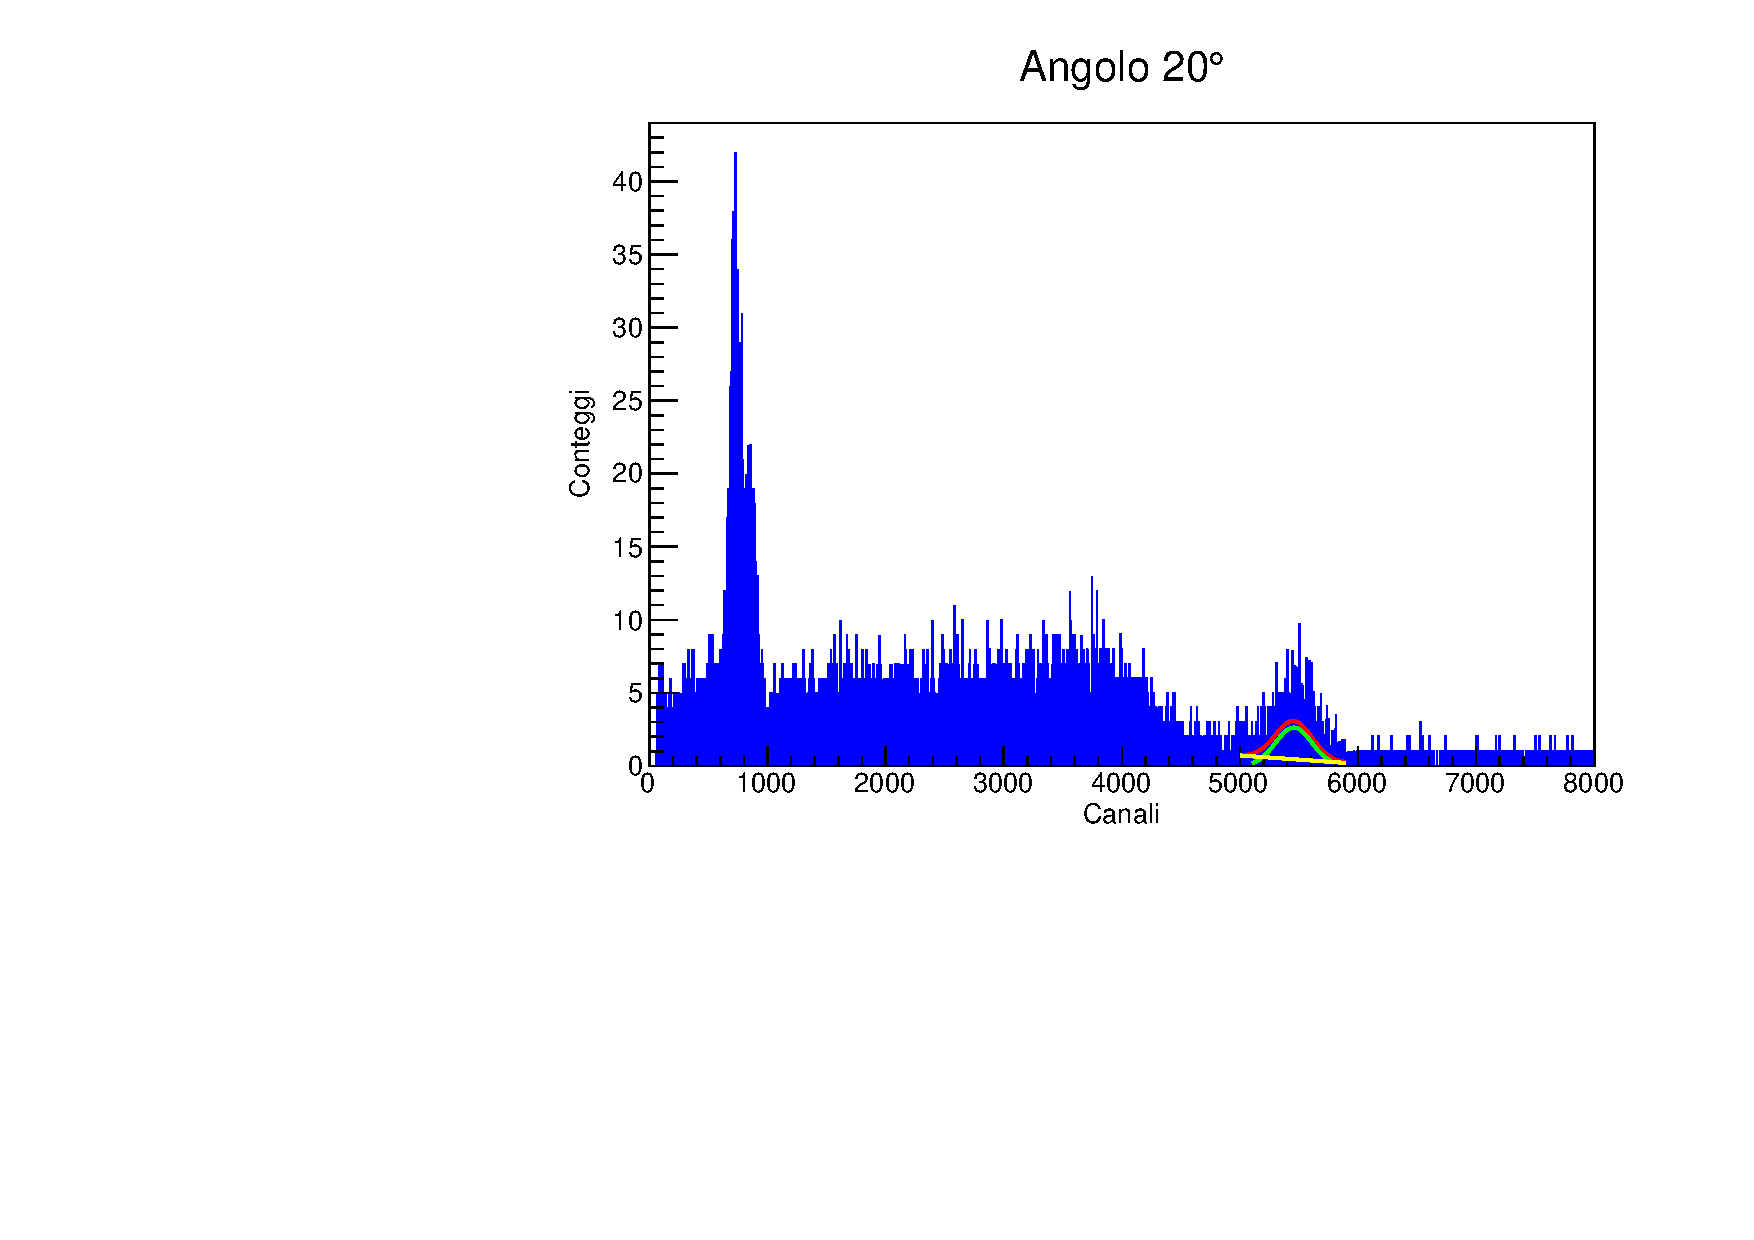
\includegraphics[width=12cm]{20finale.pdf}
\end{center}

L'ultimo grafico rappresenta il fit ottenuto dalla differenza tra i due spettri mostrati in precedenza. In rosso si ha la prima gaussiana ottenuta tramite un fit dell'istogramma; in giallo si ha un polinomio del primo grado che rappresenta il rumore di fondo; in verde si ha la gaussiana finale data dalla differenza della due funzioni precedentemente descritte.

\vspace{1cm}
I valori ottenuti sono:
\begin{align*}
\frac{d\sigma}{d\Omega} =(7,3&\pm1,4)\times10^{-26} cm^2 \\
Ch_{picco}&=5424\pm8
\end{align*}

\vspace{3cm}
\subsection{Angolo 30$^\circ$}
A seguito della misura a 30$^\circ$, abbiamo osservato la presenza di un picco non atteso nello spettro rilevato. Abbiamo quindi deciso di fare un'analisi approfondita del fondo facendo una misura di circa una settimana in assenza di targhetta. Nello spettro relativo al fondo è stato effettivamente osservato il picco cercato: probabilmente questo picco è dato dalla riflessione di fotoni su una mattonella di piombo. Lo spettro relativo ai 30$^\circ$ è stato quindi analizzato sottraendo il fondo rilevato. Dato che i tempi di acquisizione del segnale e del fondo erano differenti, è stato necessario normalizzare il fondo in funzione del tempo di esecuzione dello spettro. Una volta ottenuto il grafico rappresentante la differenza tra le misure e il fondo, è stato analizzato il picco osservato.
\begin{figure}[!htp]
\centering
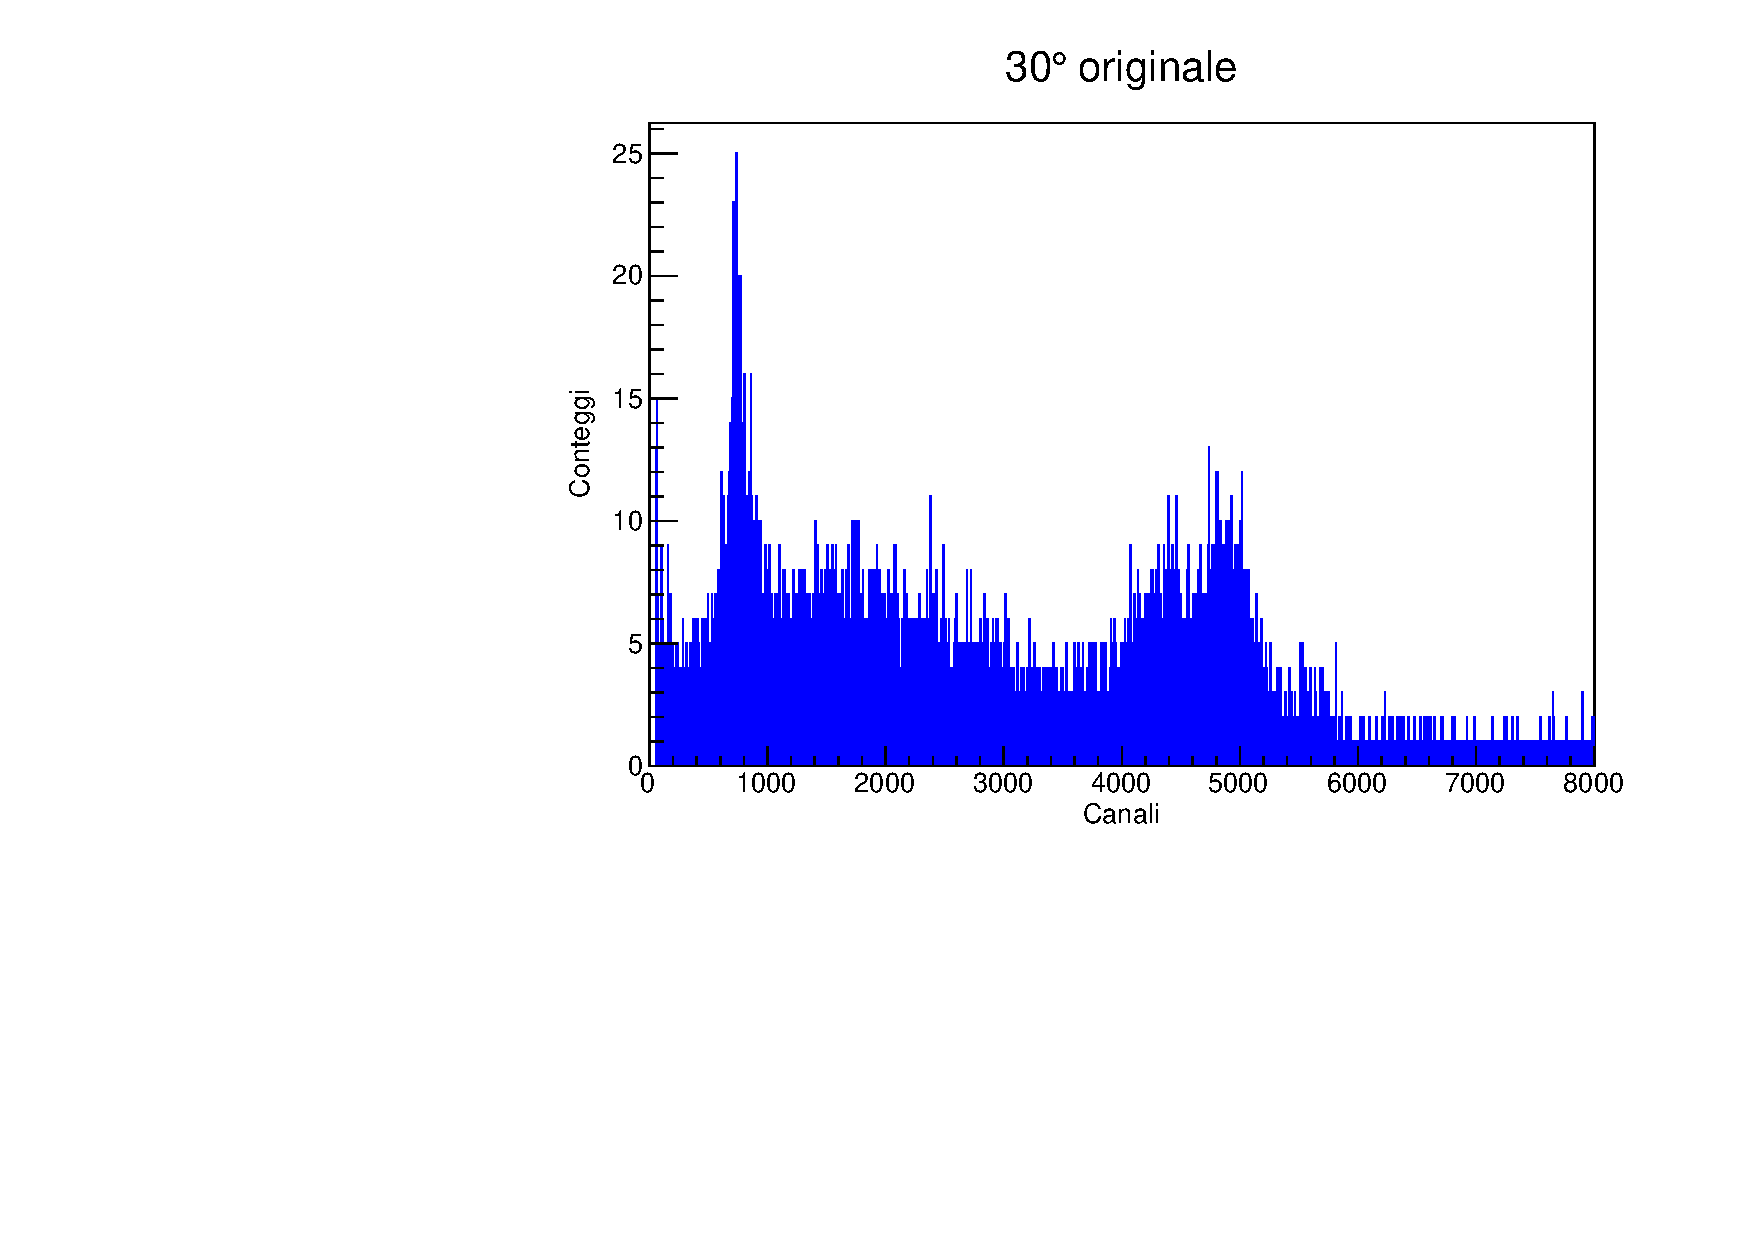
\includegraphics[width=12cm]{30originale.pdf}
\caption{Spettro rilevato a 30$^\circ$}
\end{figure}
\begin{figure}[!htp]
\centering
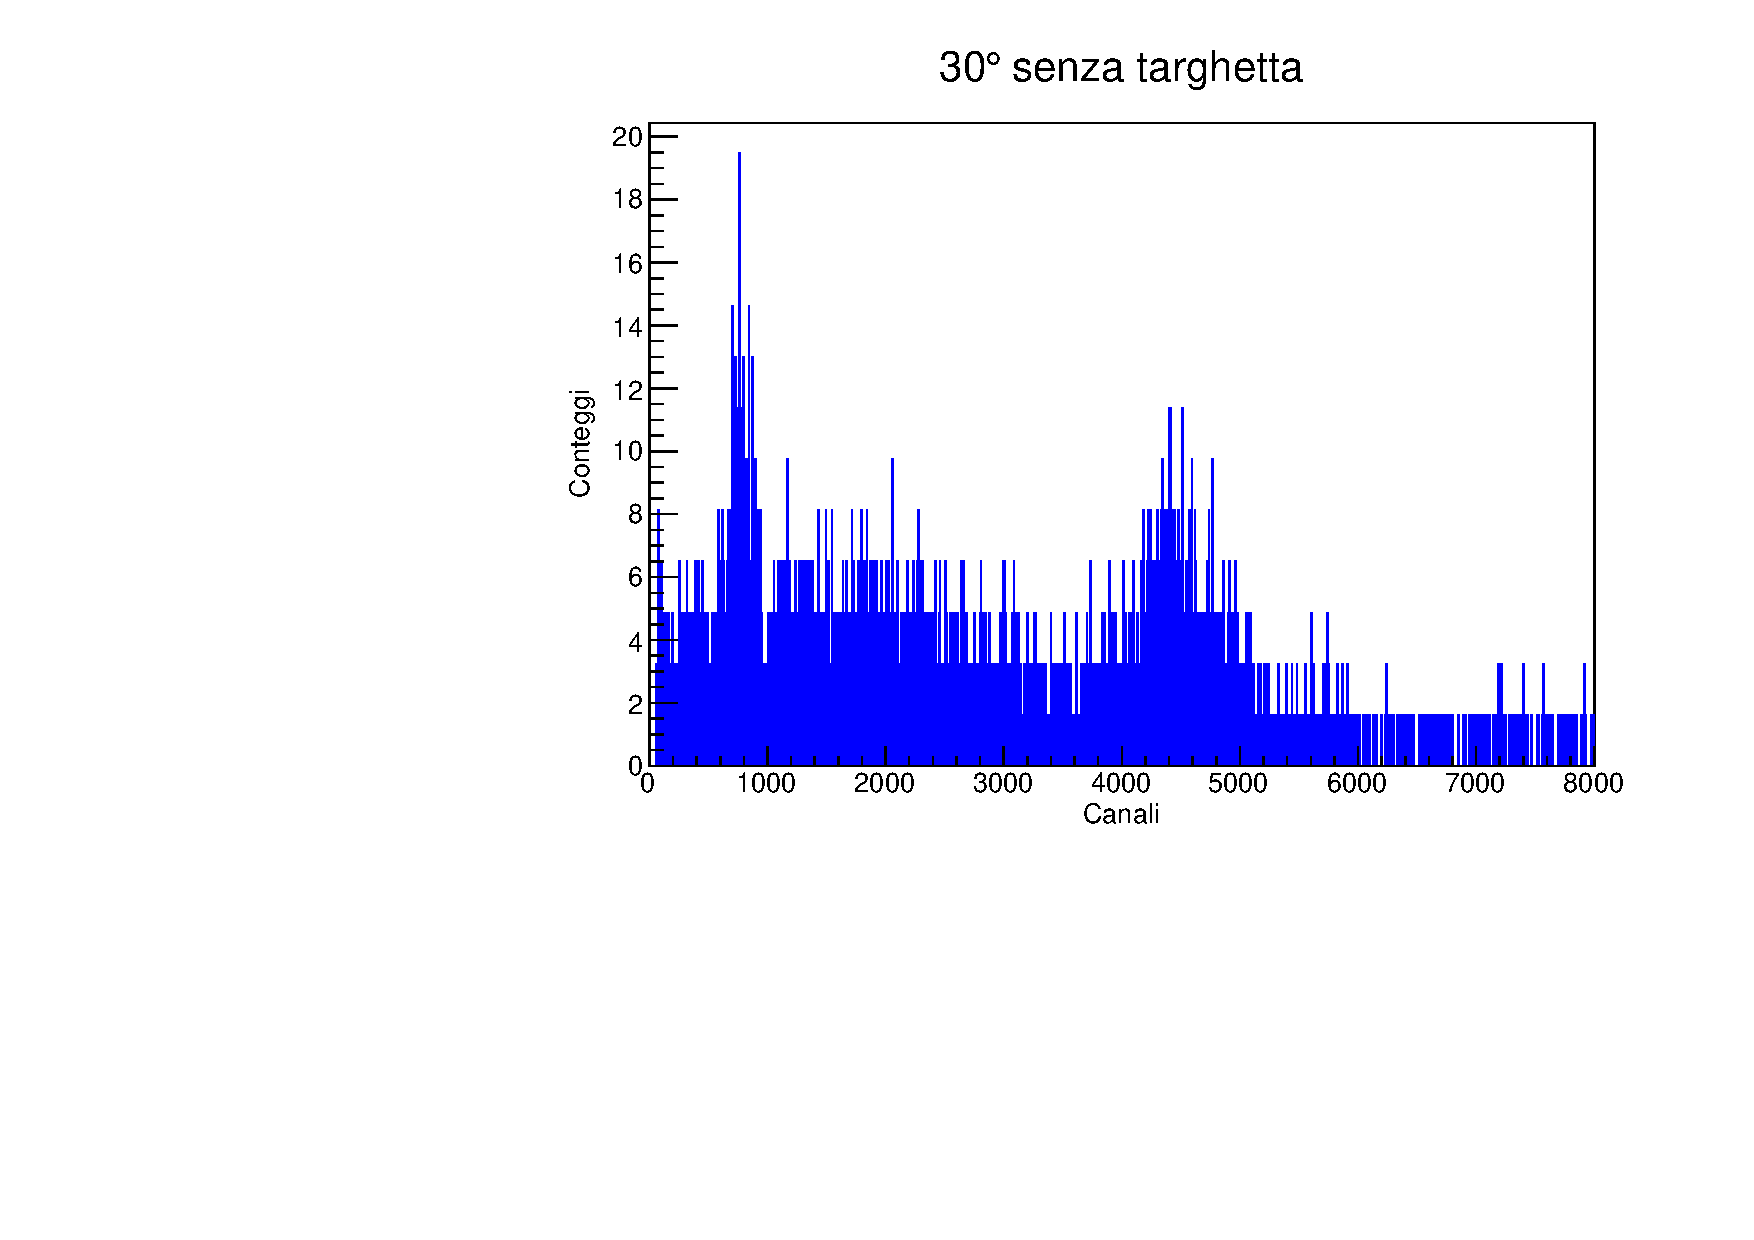
\includegraphics[width=12cm]{30notarghet.pdf}
\caption{Spettro di fondo rilevato a 30$^\circ$}
\end{figure}
\begin{figure}[!htp]
\centering
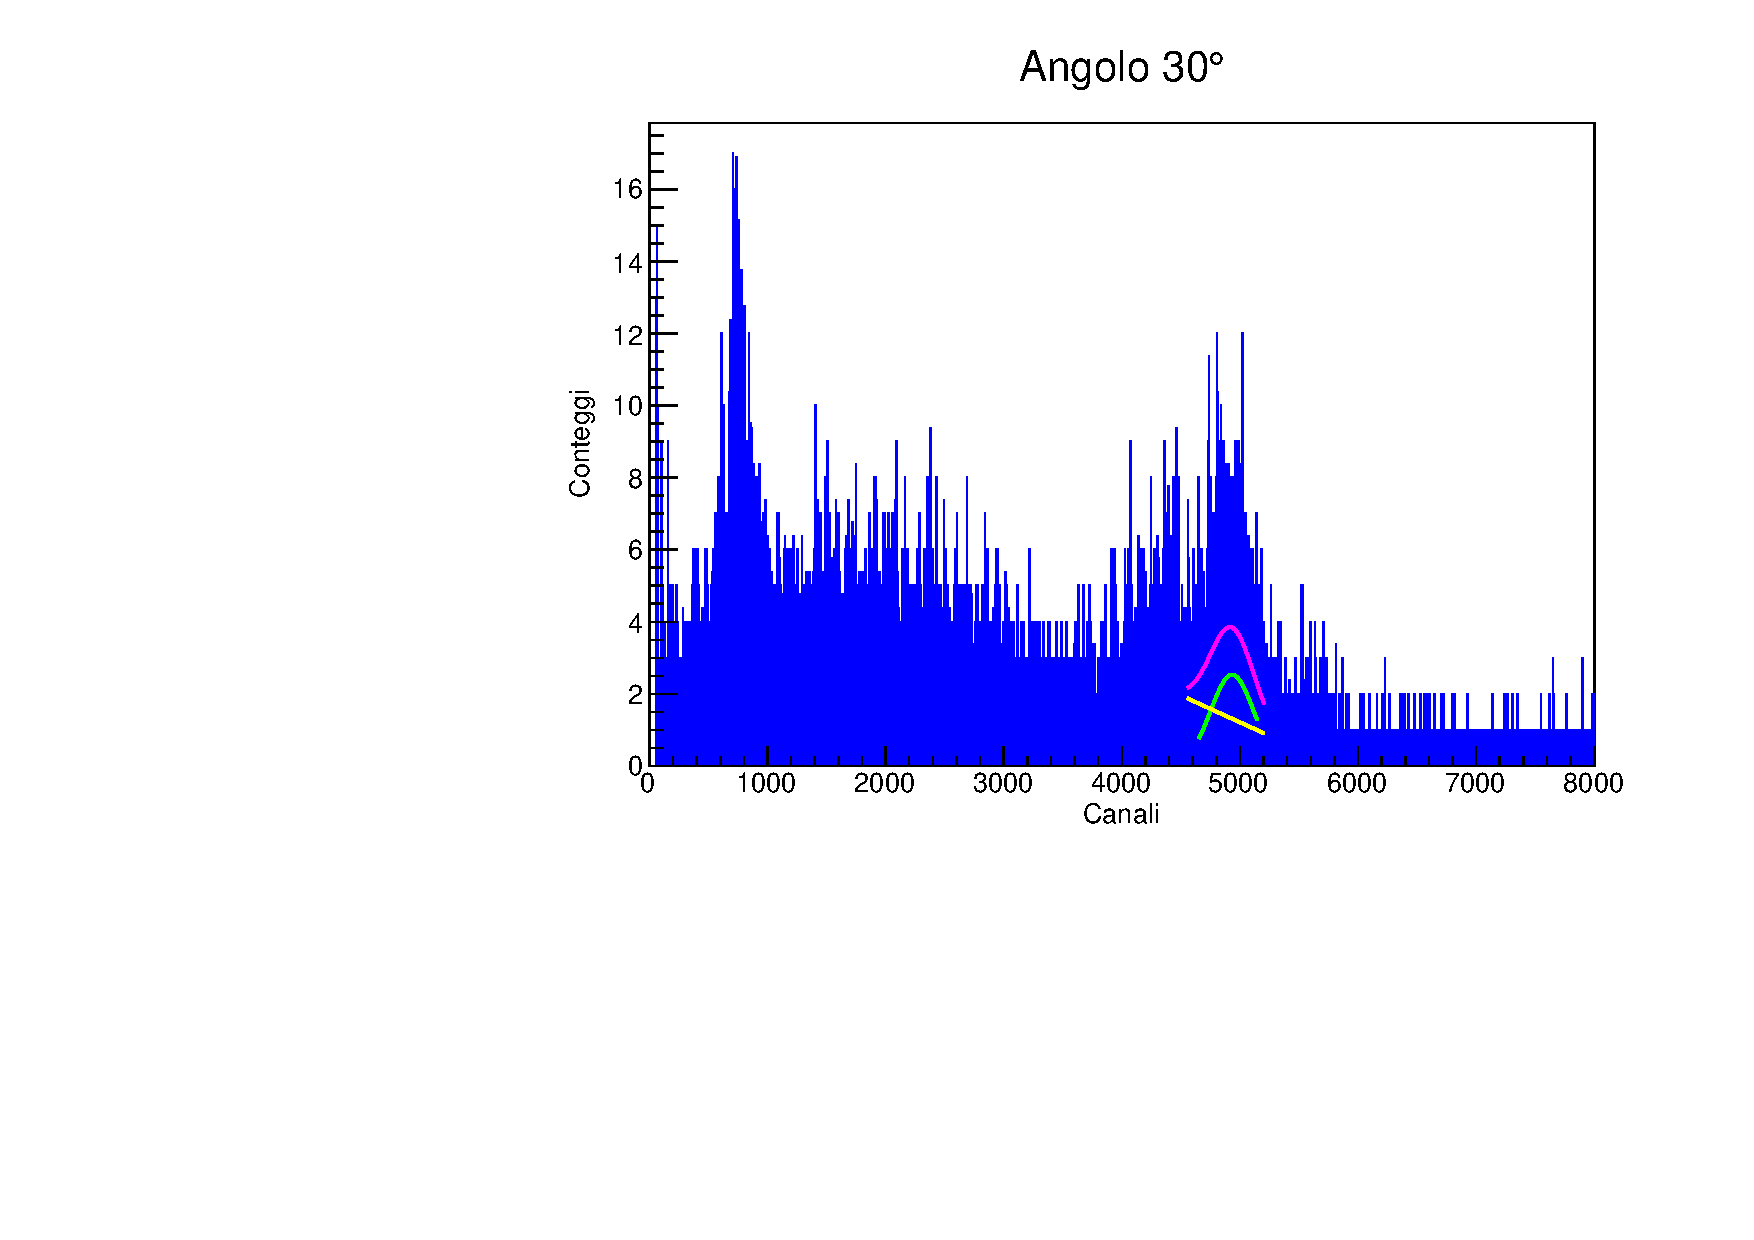
\includegraphics[width=12cm]{30finale.pdf}
\caption{Spettro finale a 30$^\circ$ ottenuto dalla differenza tra lo spettro rilevato e il fondo con fit gaussiano}
\end{figure}
\begin{figure}[!htp]
\centering
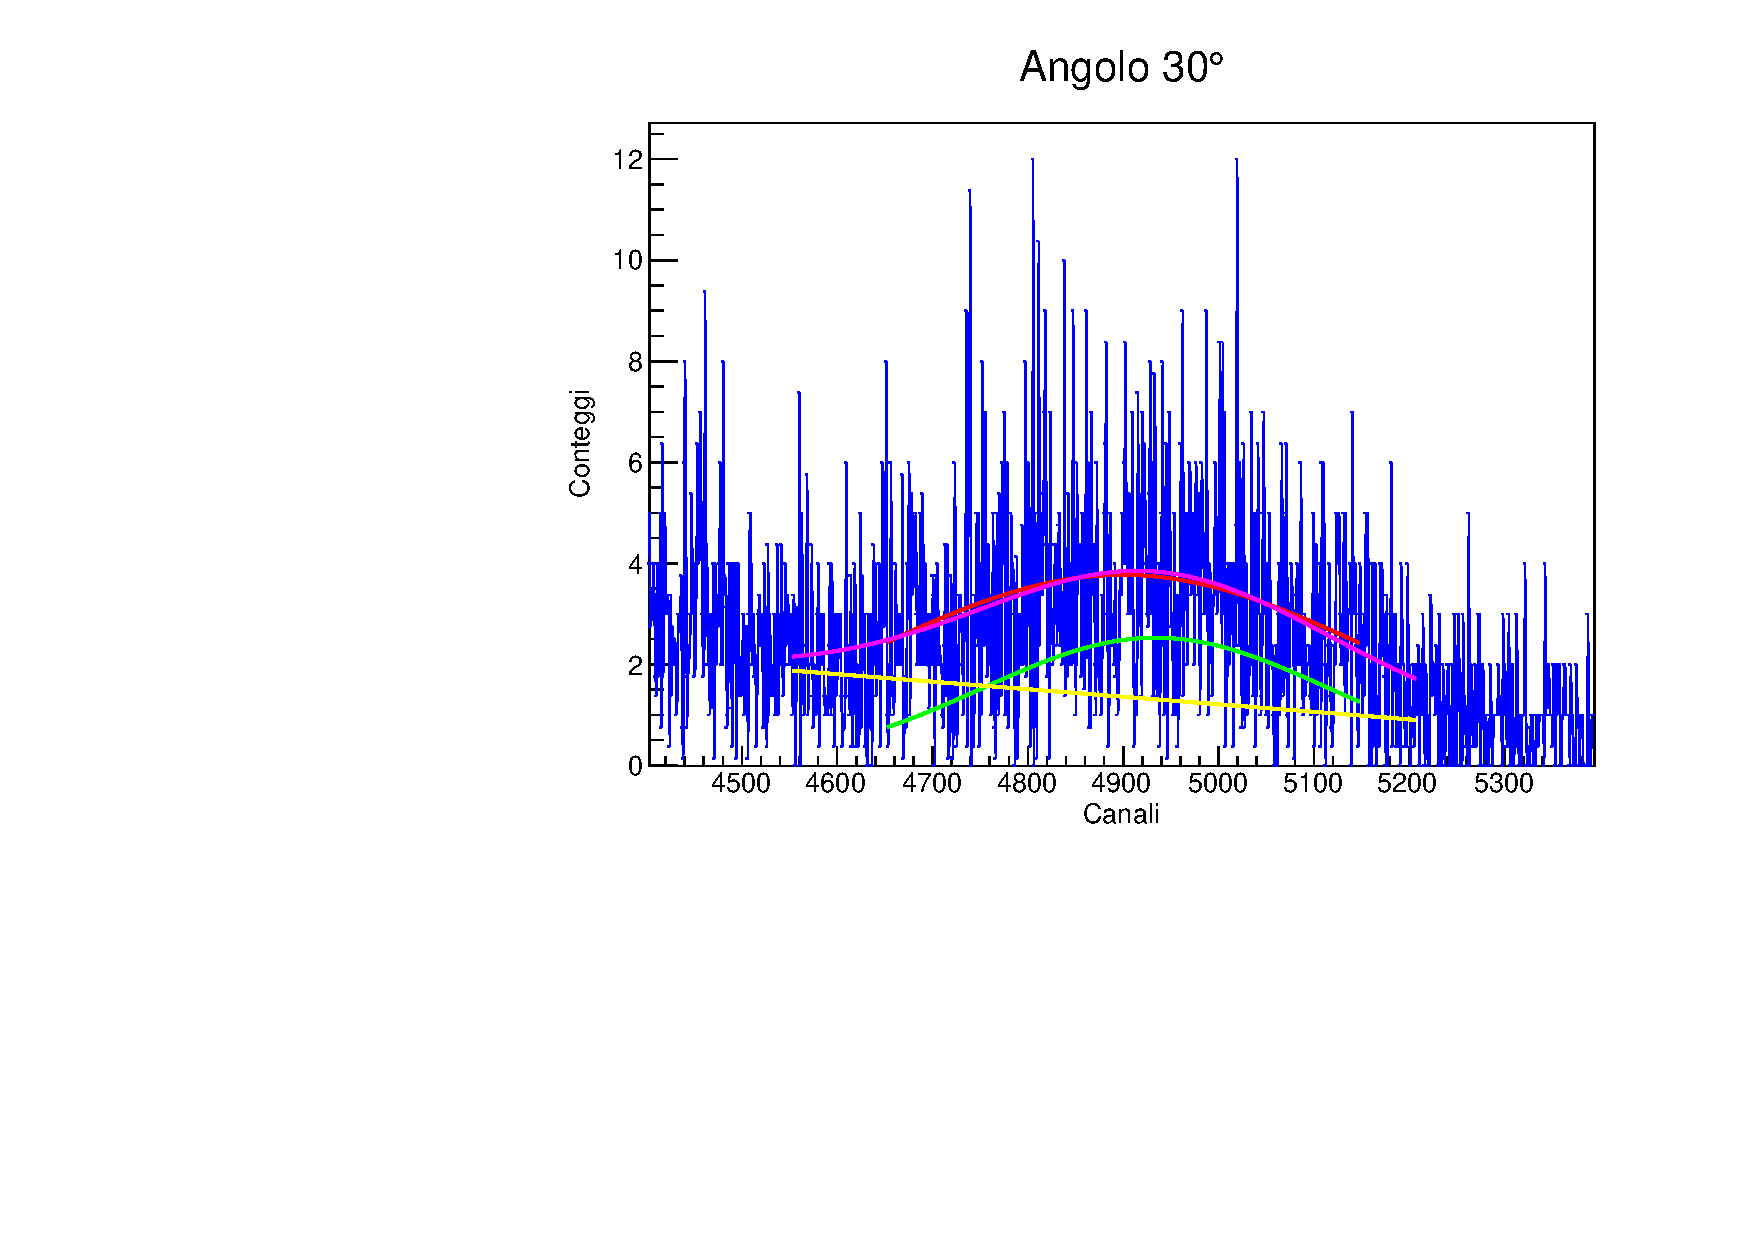
\includegraphics[width=12cm]{30zoom.pdf}
\caption{Zoom del fit finale}
\end{figure}

\vspace{10cm}
I valori ottenuti sono:
\begin{align*}
\frac{d\sigma}{d\Omega} =(5,53&\pm0,95)\times10^{-26} cm^2 \\
Ch_{picco}&=4934\pm15
\end{align*}
\vspace{2cm}

\subsection{Angolo 45$^\circ$}

\newpage
\subsection{Angolo 60$^\circ$}
Per questa misura abbiamo proceduto ad una analisi del fondo: abbiamo preso misure di circa quattro giorni in assenza di targhetta. Il fondo osservato è stato poi sottratto allo spettro raccolto. Facendo l'usuale analisi dati con Root risultava impossibile fittare correttamente il picco: invece che utilizzare l'usuale istogramma, abbiamo provato a fittare il picco con l'opzione \textit{graph} e questo ci ha permesso di ottenere una gaussiana che ben approssima il picco osservato.
\begin{figure}[!htp]
\centering
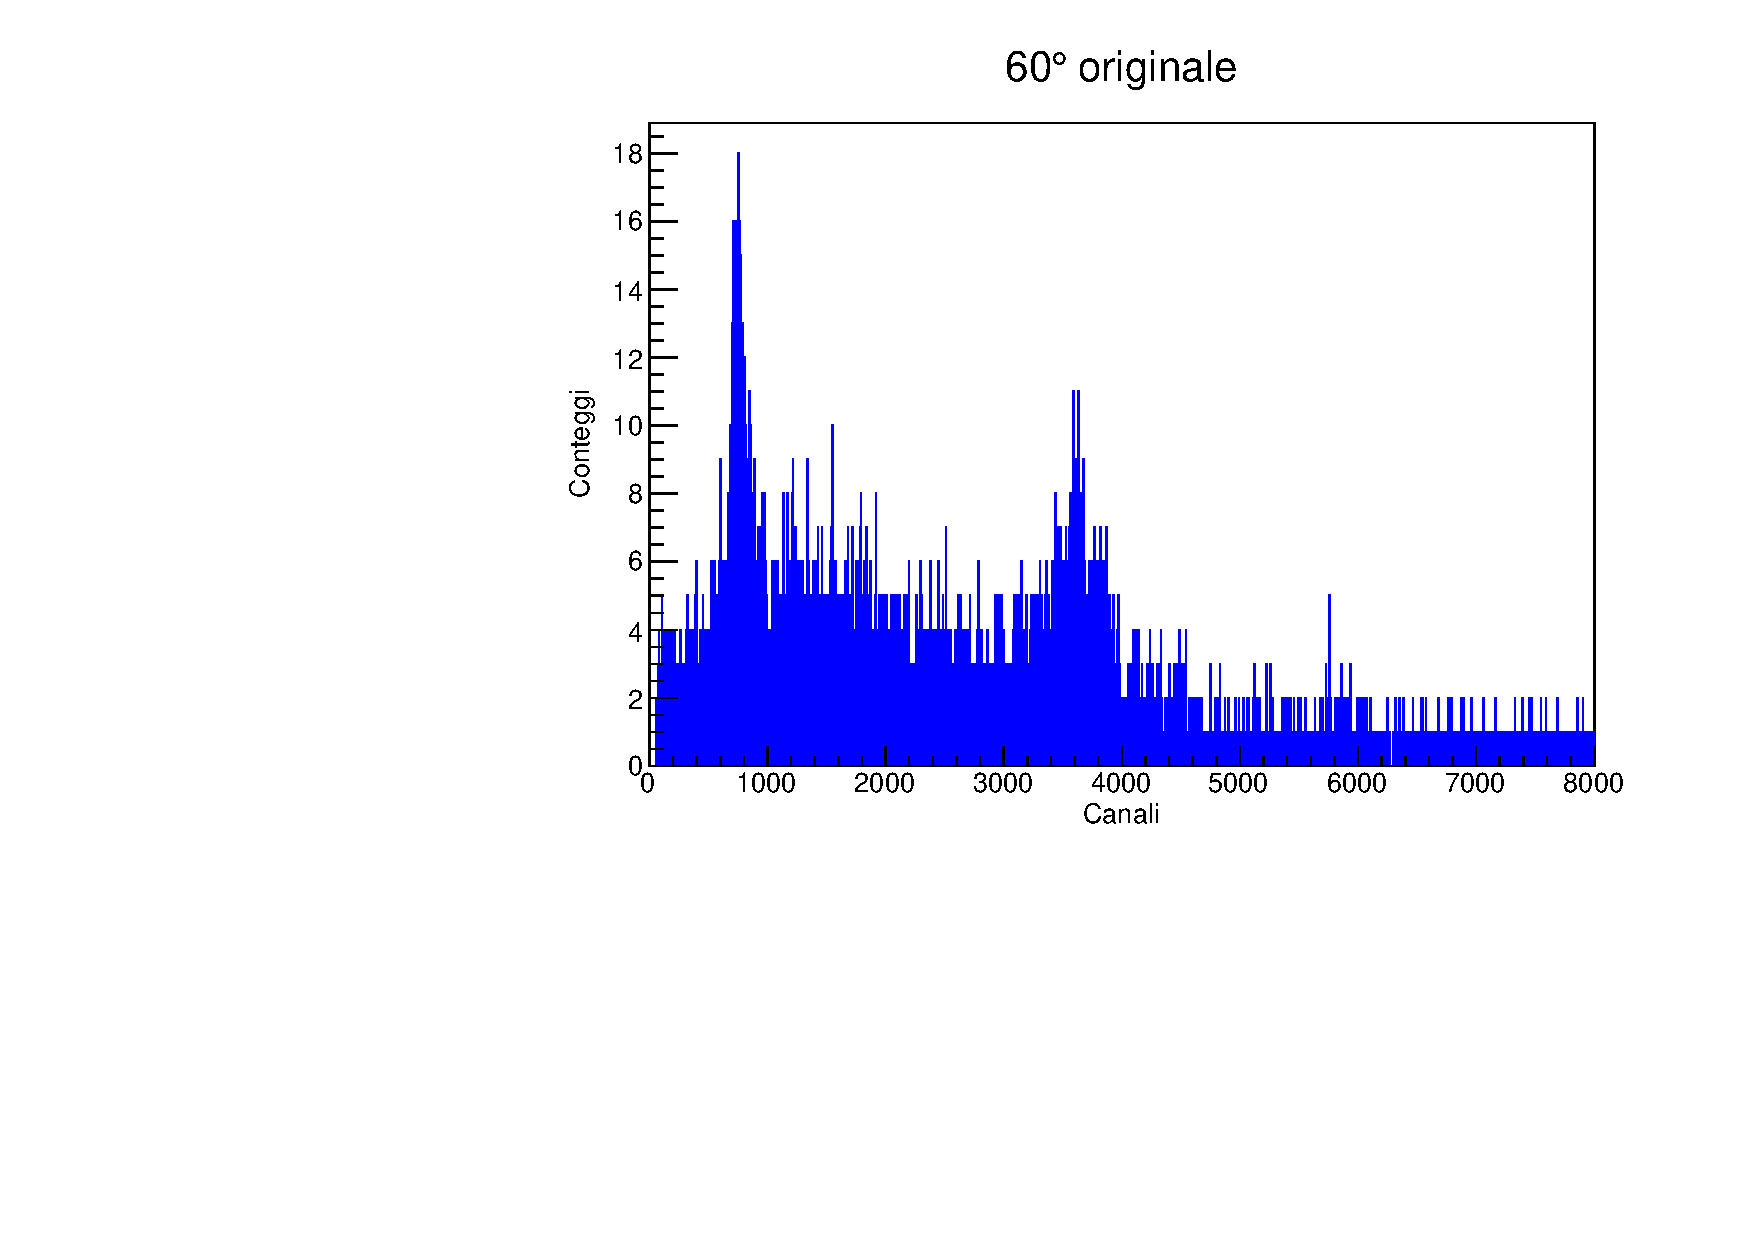
\includegraphics[width=12cm]{60originale.pdf}
\caption{Spettro rilevato a 60$^\circ$}
\end{figure}
\begin{figure}[!htp]
\centering
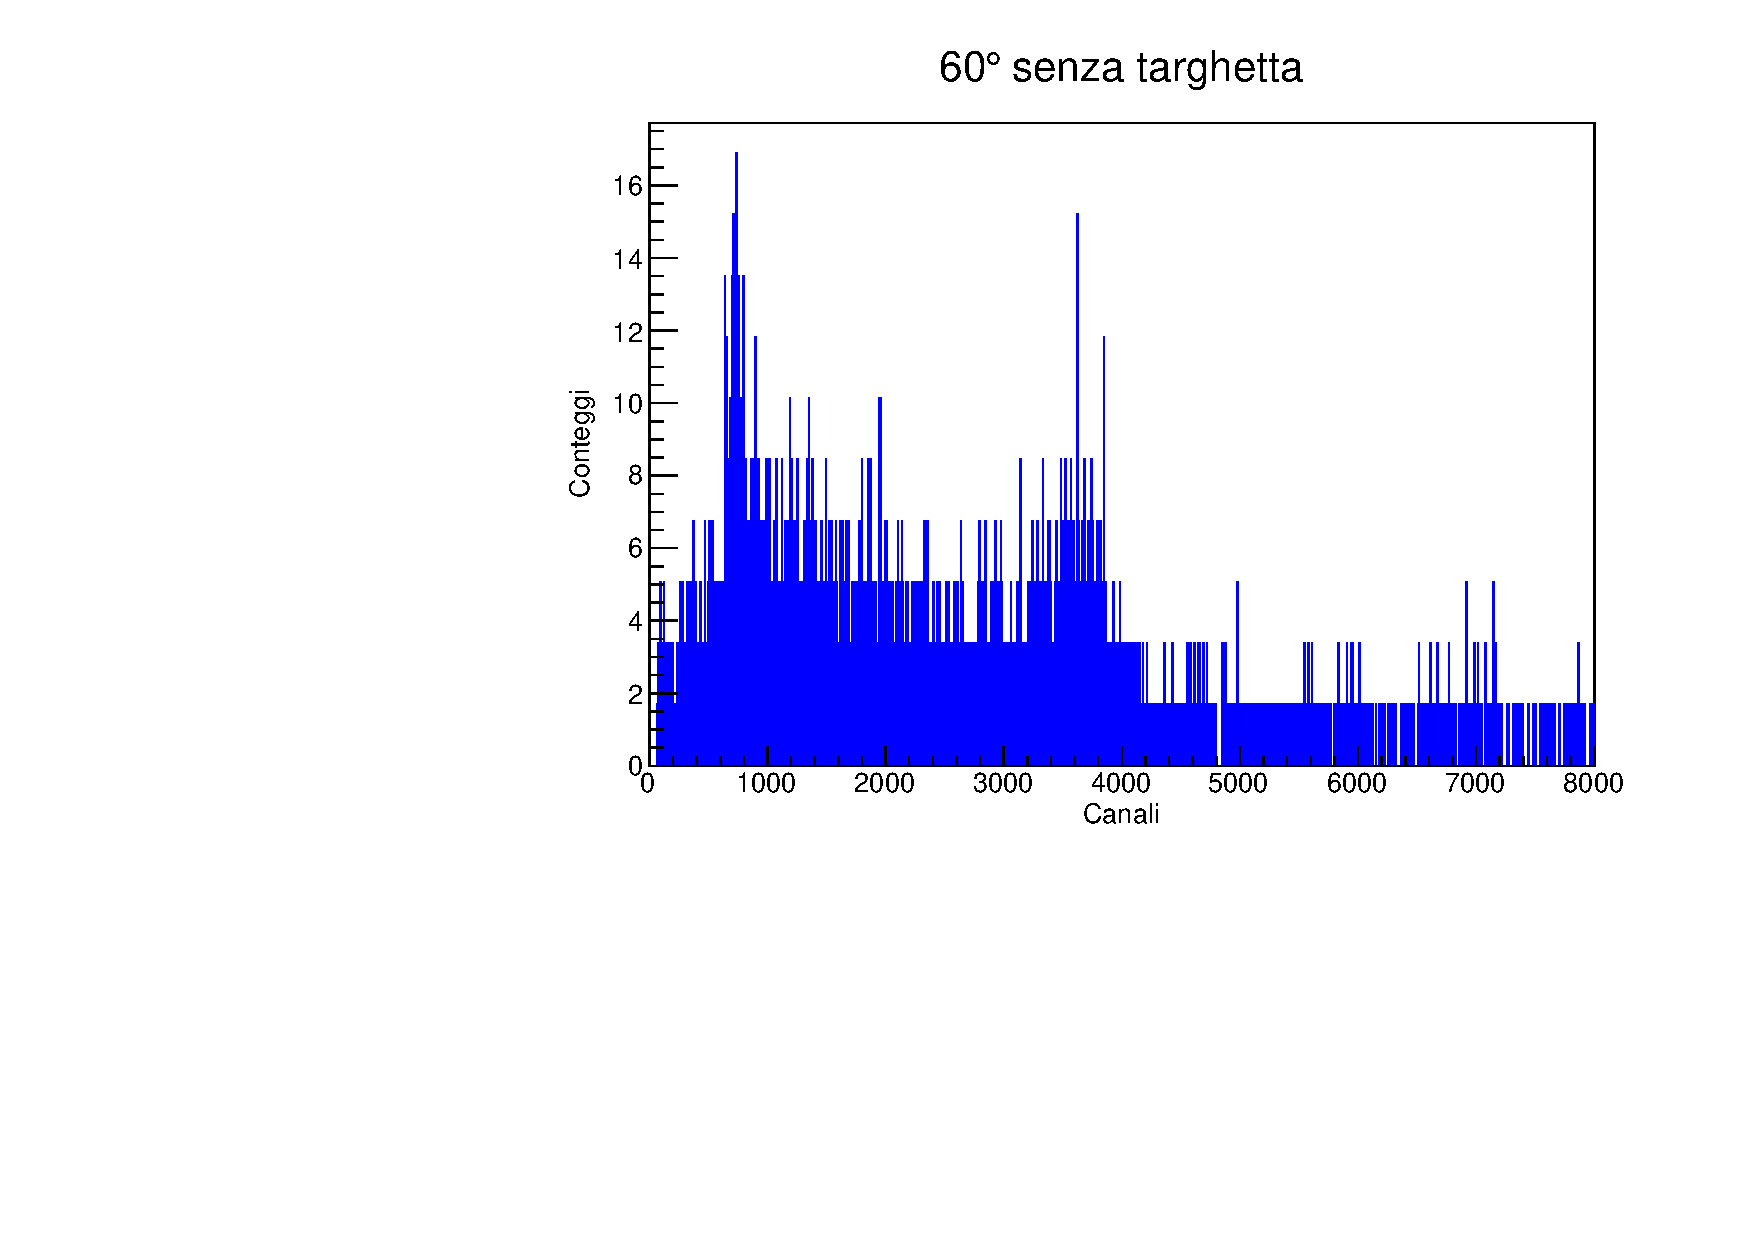
\includegraphics[width=12cm]{60notarget.pdf}
\caption{Spettro di fondo rilevato a 60$^\circ$}
\end{figure}
\begin{figure}[!htp]
\centering
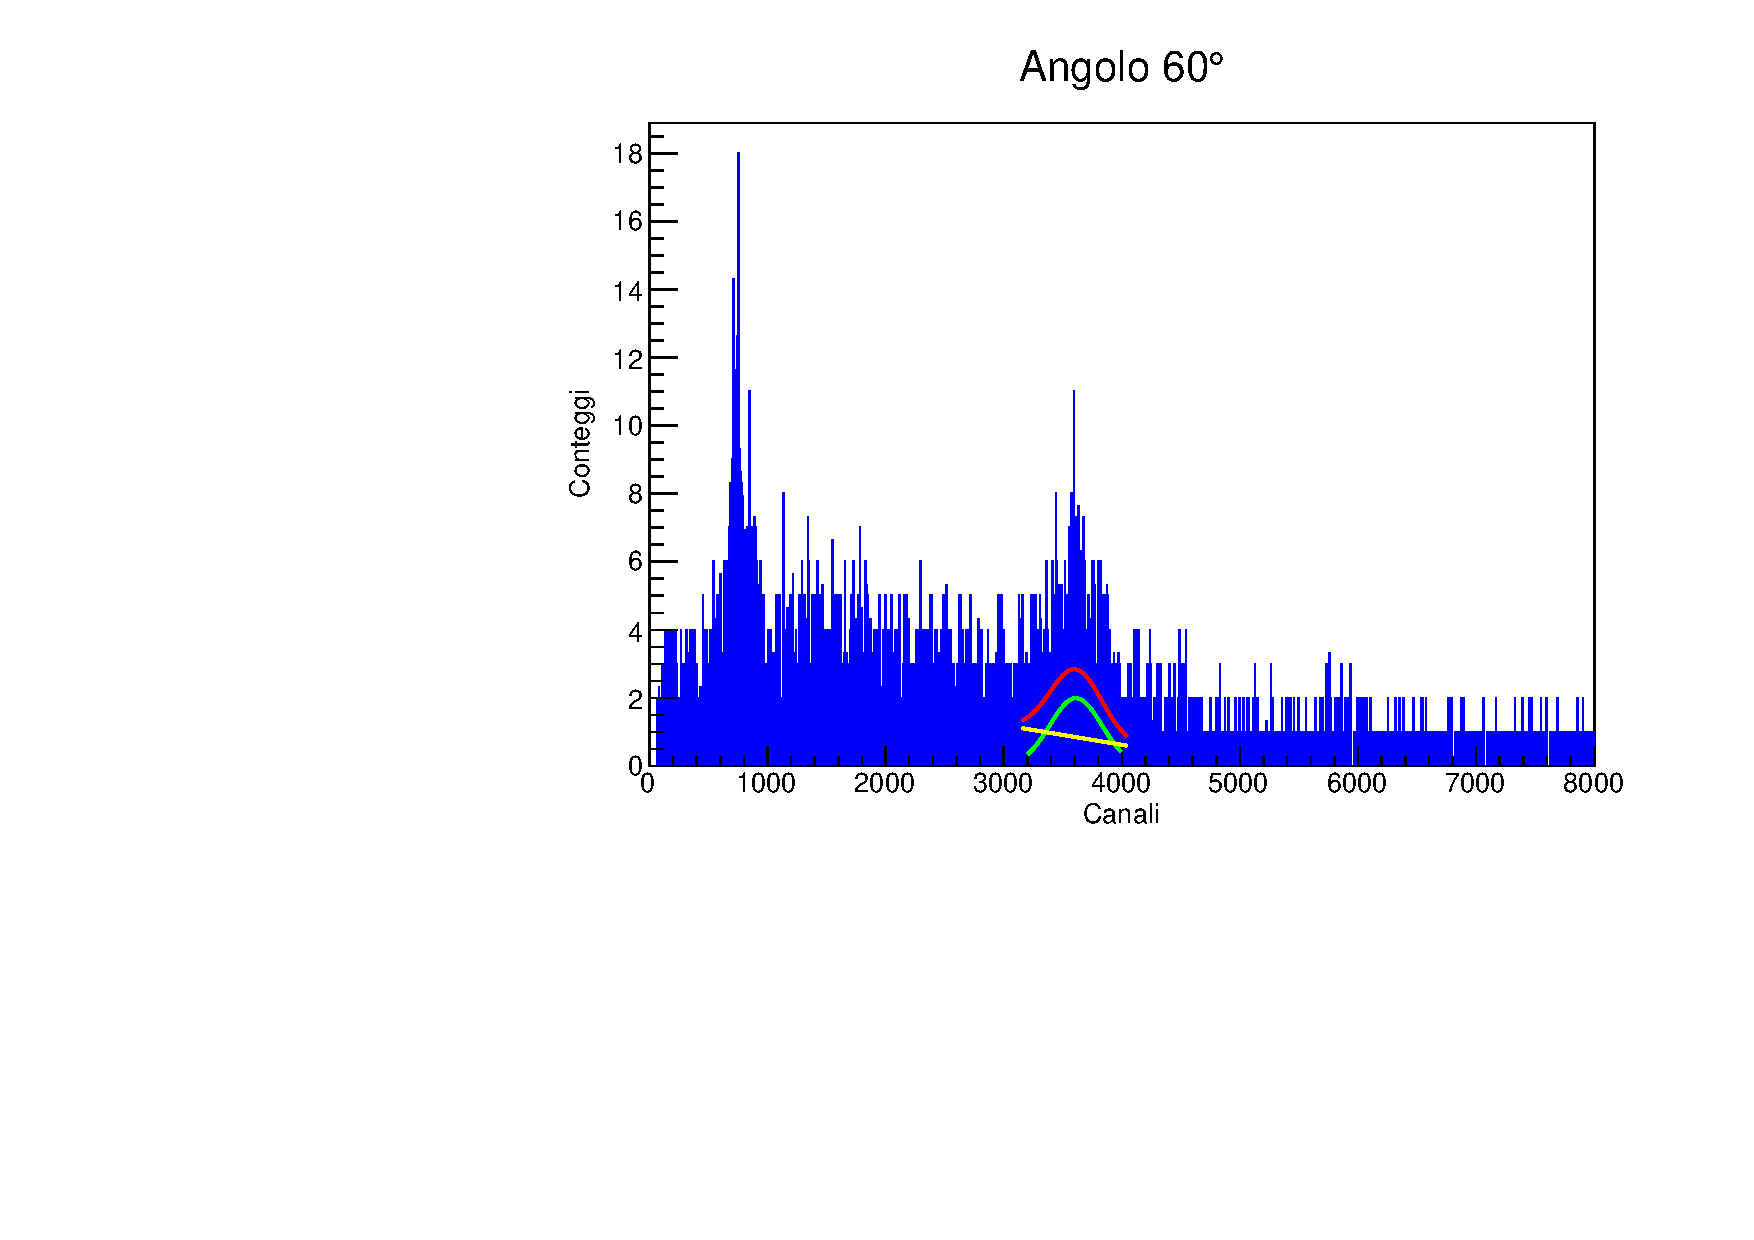
\includegraphics[width=12cm]{60finale.pdf}
\caption{Spettro finale a 60$^\circ$ ottenuto dalla differenza tra lo spettro rilevato e il fondo con fit gaussiano}
\end{figure}

\vspace{5cm}
I valori ottenuti sono:
\begin{align*}
\frac{d\sigma}{d\Omega} =(3,1&\pm0,9)\times10^{-26} cm^2 \\
Ch_{picco}&=3611\pm13
\end{align*}


\newpage
\section {Analisi dati}
\subsection{Sezione d'urto e legge di Klein-Nishina}
Gli errori indicati sono stati tutti ricavati tramite una propagazione degli errori. Gli errori sull'attività della sorgente e sul tempo di esecuzione sono stati considerati trascurabili. Abbiamo scelto di fissare un errore sull'angolo di scattering di 2$^\circ$. Le distanza tra i vari elementi dell'apparato misurate con una riga hanno un'incertezza al millimetro, mentre i diametri dei rilevatori, essendo stati misurati col calibro, hanno un'incertezza pari a 0,50mm. Gli errori relativi a grandezza ricavate con fit sono quelle indicate dal fit stesso. 
I dati ricavati e analizzati nello studio della sezione d'urto sono :
\vspace{0,5cm}
\begin{center}
    \centering
    \begin{tabular}{cccccc}
    \hline
    $\theta$($^\circ$)& Integral& $t_{es}$(s)& $\Delta$n&  $\frac{d\sigma}{d\Omega}(cm^{2})$$\cdot$$10^{-26}$\\
    \hline\hline
    20$^\circ$ & 973$\pm$144& 162442& 0,0060$\pm$0,0009&  7,3$\pm$1,4\\
    30$^\circ$& 2144$\pm$267& 443128& 0,005$\pm$0,006&  5,53$\pm$0,95\\
    45$^\circ$& & & & \\
    60$^\circ$& 923$\pm$250& 355345& 0,0026$\pm$0,0007&  3,1$\pm$0,9\\
    \hline
    \end{tabular}
    \end{center}
    \vspace{0,5cm}
L'errore che ha il maggiore peso nella misura della sezione d'urto è dato dall'errore sull'integrale della gaussiana. Questo avrebbe potuto essere abbattuto da un elevato numero di misure che avrebbe comportato un fit gaussiano più corretto. Tuttavia, a causa dei pochi dati raccolti, l'errore finale individuato risulta essere, in percentuale, piuttosto elevato, soprattutto nella misura a $60^\circ$.\newline
Riportiamo ora i valori tabulati per il rapporto delle efficienze $\frac{e(CeBr_{3},E')}{e(CeBr_{3},E)}$ del rivelatore B al variare dell'angolo utilizzati nel calcolo della sezione d'urto. I valori di K indicati in tabella sono stati calcolati per uno spessore del bersaglio di 0,24cm a partire da coefficienti di attenuazione efficaci $\lambda'$ e $\lambda''$ tabulati per il piombo in funzione dell'angolo di scattering. Questi ultimi sono generalmente espressi in unità di spessore equivalente (g/$cm^{2}$): per convertirli in lunghezze occorre moltiplicarli per la densità ($\rho_{Pb}$=11,36g/$cm^{3}$). 

\vspace{0,5cm}
\begin{center}
\centering
    \begin{tabular}{ccc}
    \hline
     $\theta$($^\circ$)&  $\frac{e(CeBr_{3},E')}{e(CeBr_{3},E)}$& K(cm)\\
    \hline\hline
    20$^\circ$& 1,00 & 0,165\\
    30$^\circ$& 1,10 & 0,159\\
    45$^\circ$& 1,16& 0,149\\
    60$^\circ$& 1,27& 0,131\\
    \hline
    \end{tabular}
\end{center}
\vspace{0,5cm}
Confrontiamo ora i valori ottenuti per le sezioni d'urto con quelli teorici:   
\vspace{0,5cm}
\begin{center}
\centering
    \begin{tabular}{ccc}
    \hline
    $\theta$($^\circ$)&  ${\frac{d\sigma}{d\Omega}}_{teorico}(cm^{2})$$\cdot$$10^{-26}$& ${\frac{d\sigma}{d\Omega}}_{sperimentale}(cm^{2})$$\cdot$$10^{-26}$\\
    \hline\hline
    20$^\circ$ & 6,662&  7,3$\pm$1,4\\
    30$^\circ$& 5,452&  5,53$\pm$0,95\\
    45$^\circ$& 3,720& \\
    60$^\circ$& 2,500&  3,1$\pm$0,9\\
    \hline
    \end{tabular}
\end{center}
\vspace{0,5cm}
I valori trovati sperimentalmente risultano compatibili con quelli teorici. Il grafico relativo risulta essere:
\begin{figure}[!htp]
\centering
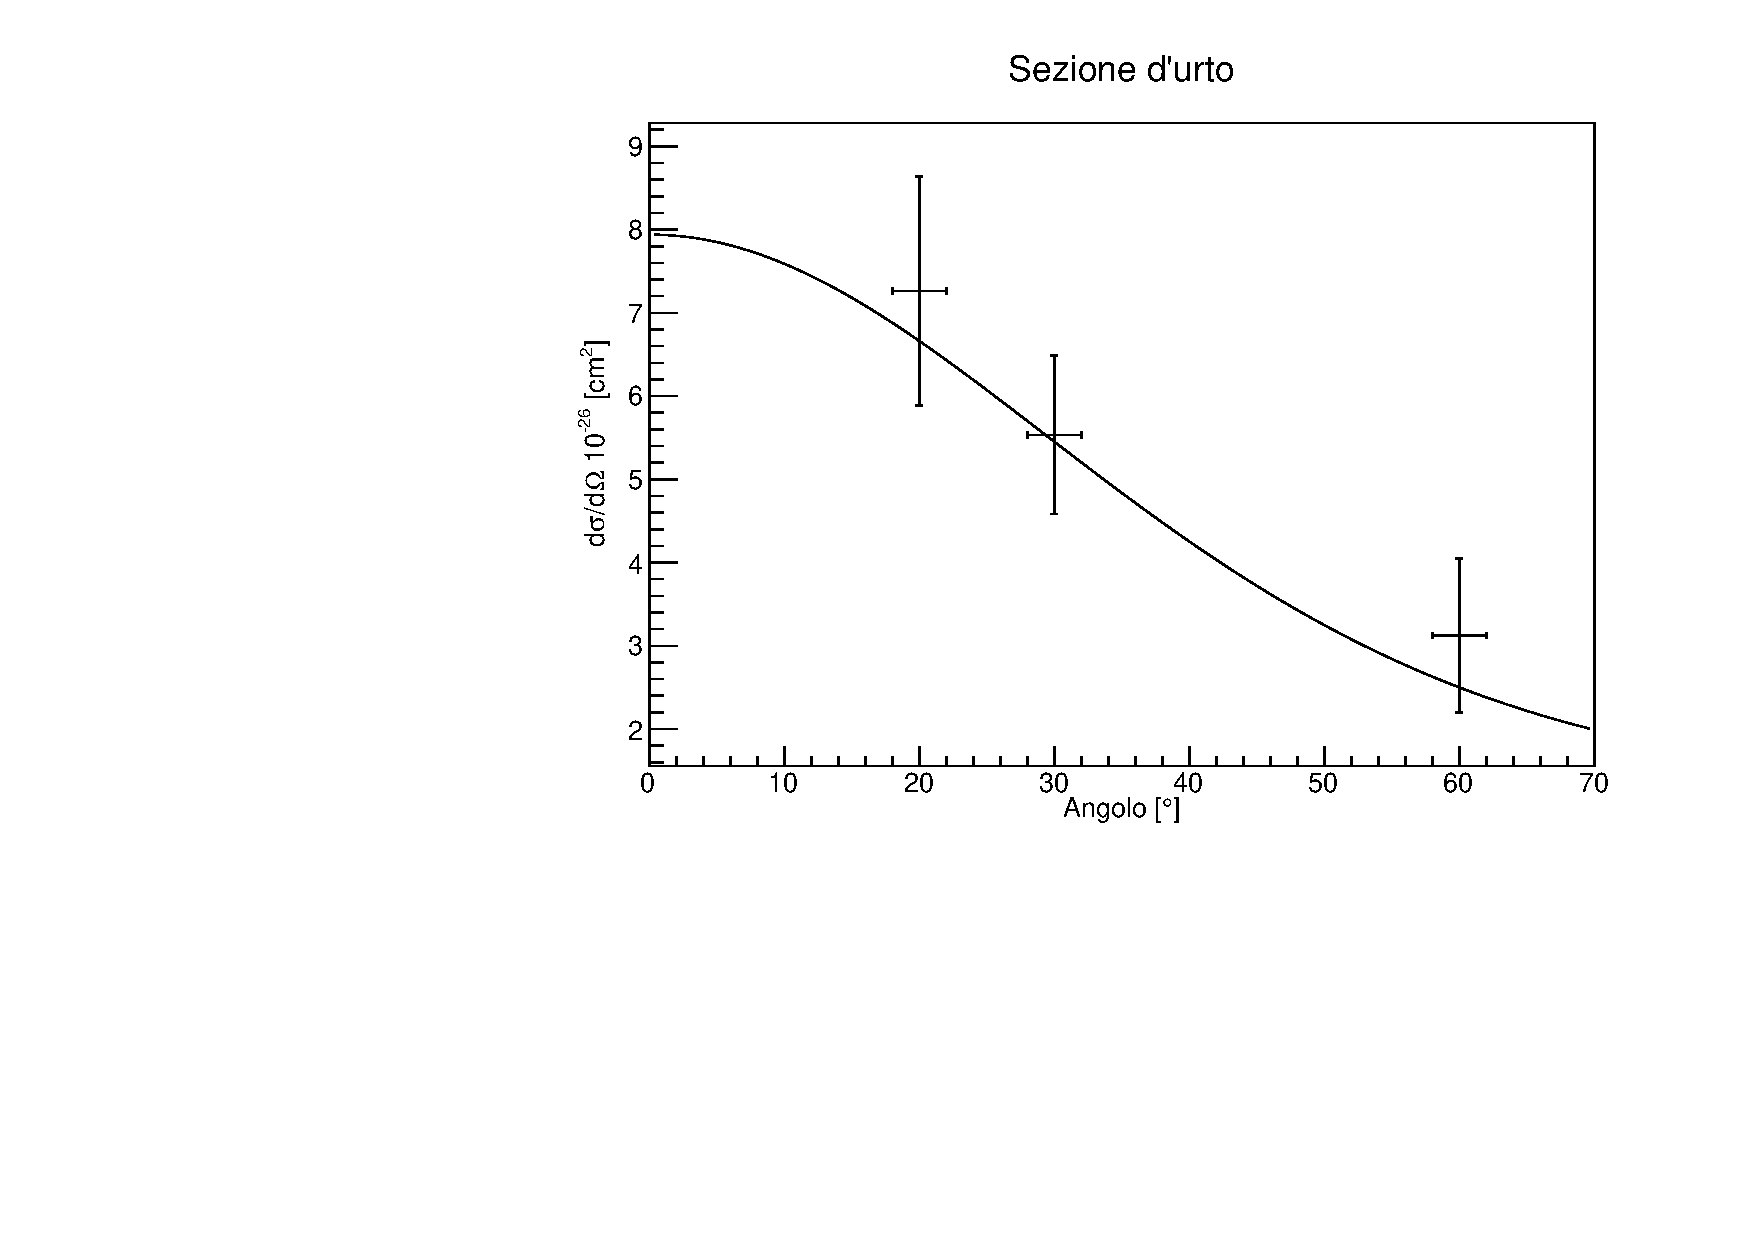
\includegraphics[width=12cm]{sezioned'urto.pdf}
\caption{Confronto tra andamento teorico (linea) e dati sperimentali della sezione d'urto al variare dell'angolo}
\end{figure}

\subsection{Verifica della legge Compton}
I dati utilizzati nello studio dell'energia del fotone diffuso sono:

\vspace{0,4cm}
\begin{center}
    \centering
    \begin{tabular}{cccc}
    \hline
    $\theta$($^\circ$)& $Ch_{picco}$ & $E'_{sperimentale}$(keV)& $E'_{teorica}$ (keV) \\
    \hline\hline
    20$^\circ$ & 5424$\pm$8 & 490$\pm$7 & 481,94\\
    30$^\circ$& 4934$\pm$15& 447$\pm$7& 450,63\\
    45$^\circ$& & & 395,24\\
    60$^\circ$& 3611$\pm$13& 329$\pm$5& 340,67\\
    \hline
    \end{tabular}
    \end{center}
\vspace{0,4cm}
I valori dell'energia del fotone diffuso sperimentali sono stati ricavati a partire dall'equazione della retta di calibrazione trovata nelle fasi preliminari dell'esperienza. \newline Il grafico ottenuto risulta essere:
\begin{figure}[!htp]
\centering
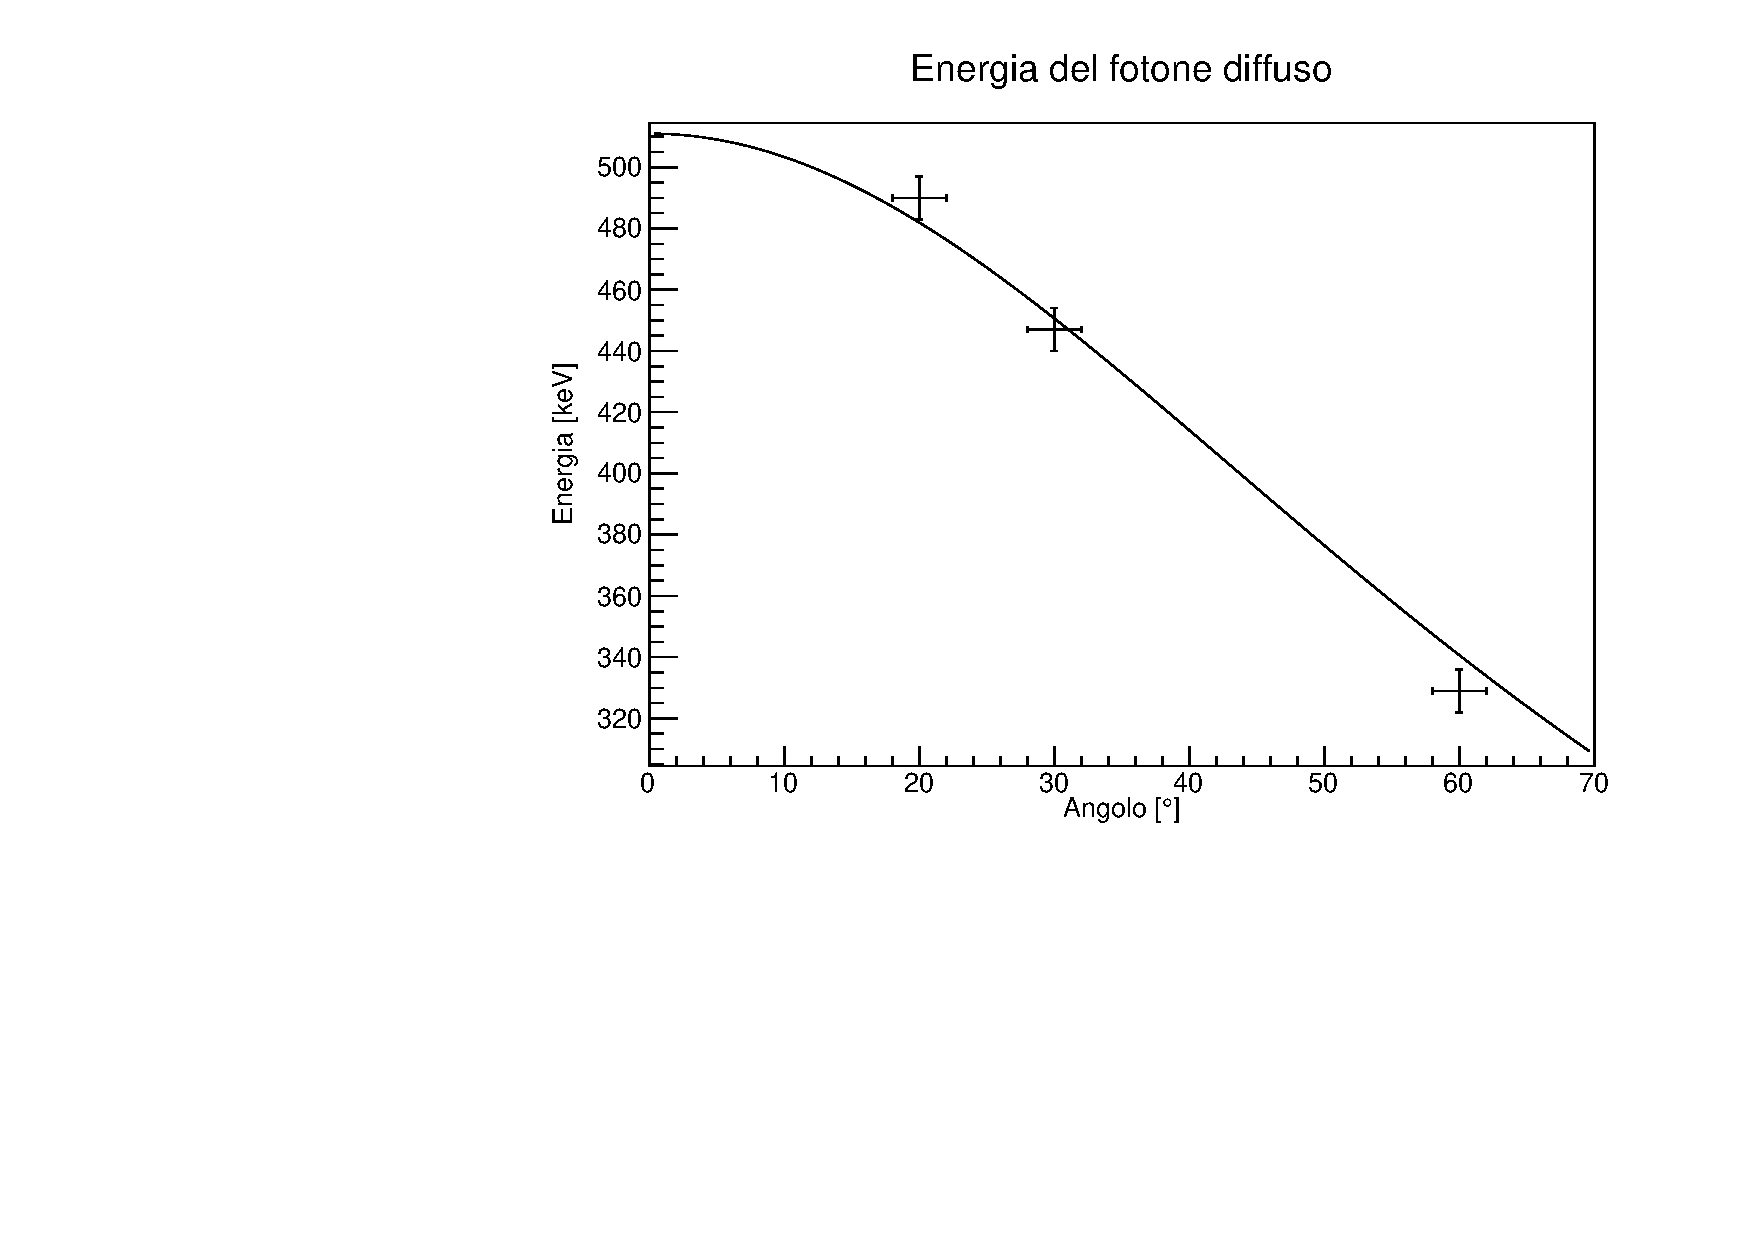
\includegraphics[width=12cm]{EnergiaFotone.pdf}
\caption{Confronto tra andamento teorico (linea) e dati sperimentali dell'energia del fotone diffuso al variare dell'angolo}
\end{figure}

\subsection{Misura della massa dell'elettrone}
Dai dati mostrati in precedenza è possibile ricavare la massa dell'elettrone. Essendo E=511keV=m$c^{2}$, sostituendo nella legge Klein-Nishina si ottiene 
\begin{equation}
E'_{\gamma}=\frac{mc^{2}}{2-cos\theta}
\end{equation}
Eseguendo un fit lineare tra E' e $\frac{1}{2-cos\theta}$, il coefficiente angolare della retta ottenuta risulta essere la massa dell'elettrone espressa in keV.

\begin{figure}[!htp]
\centering
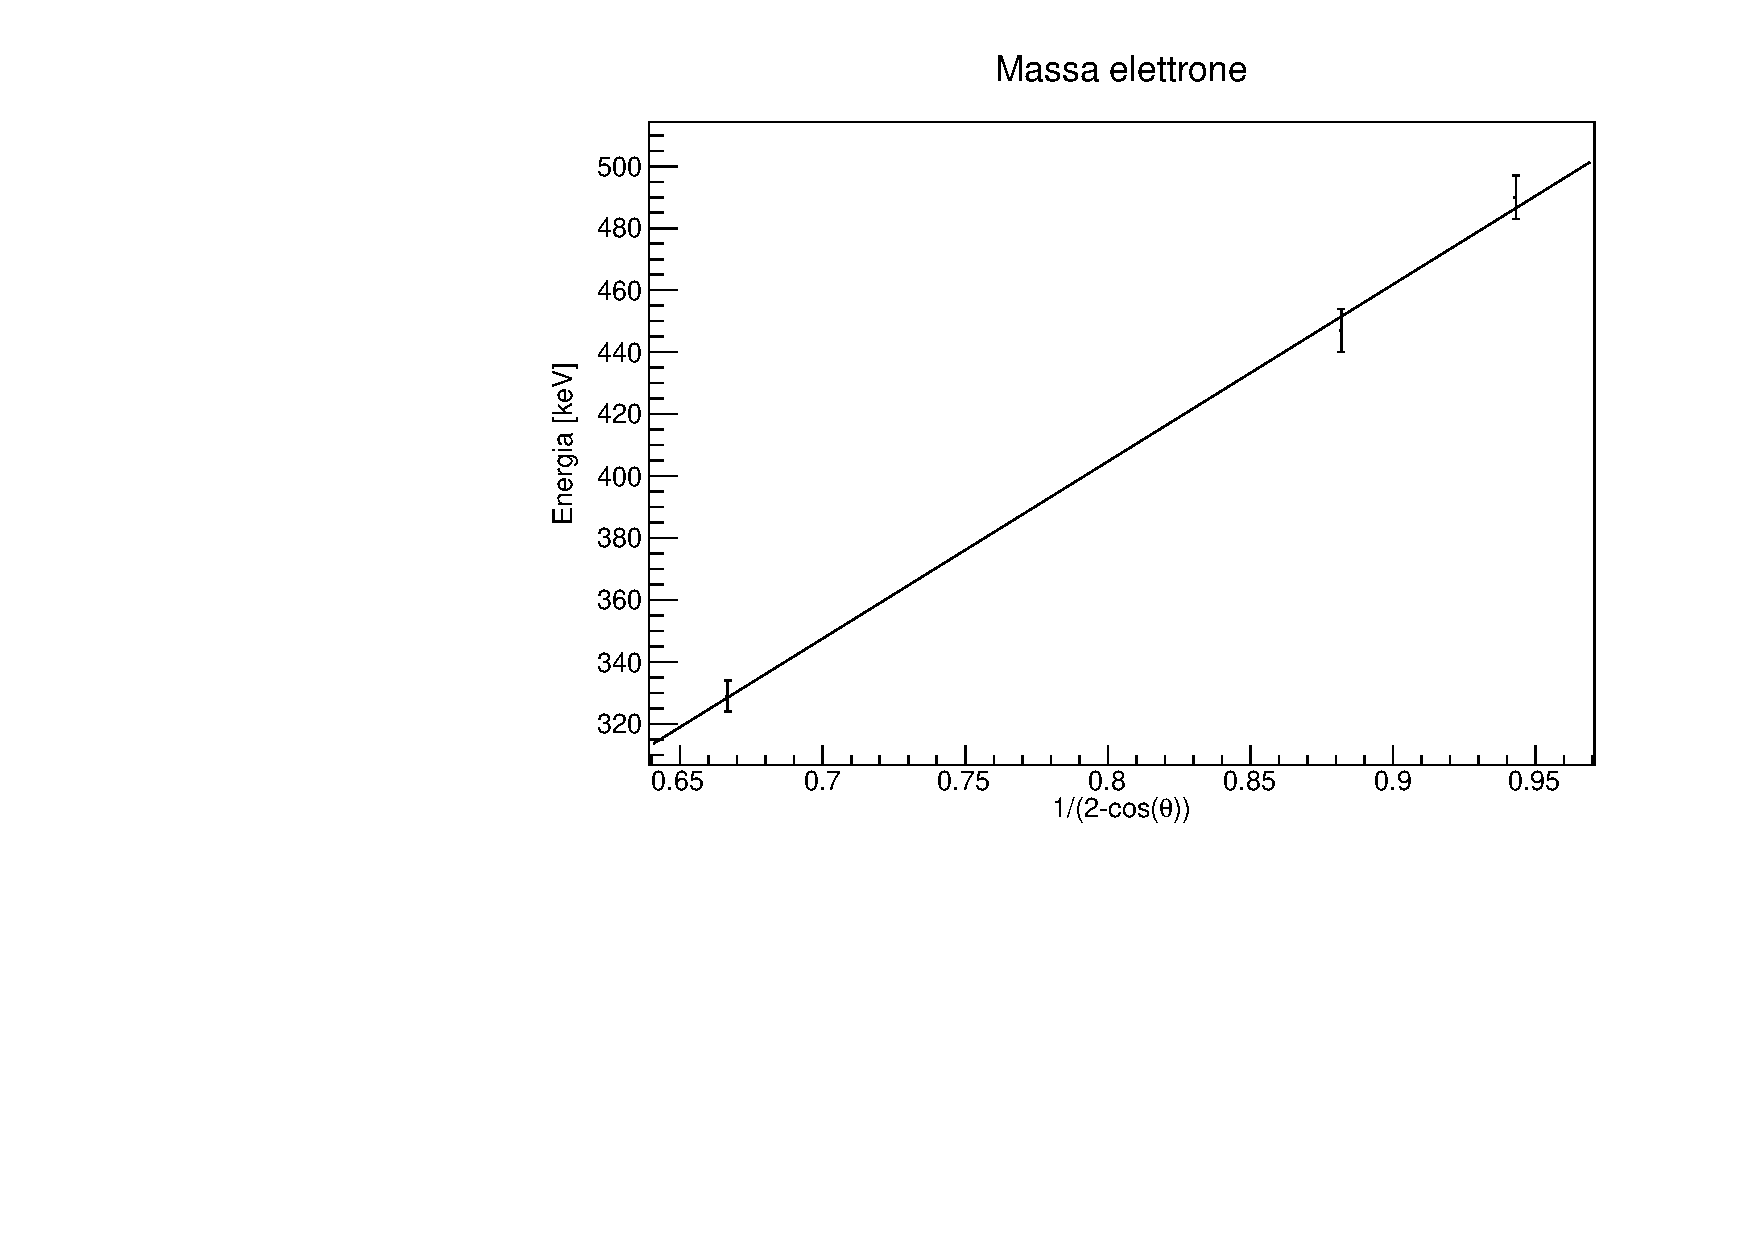
\includegraphics[width=12cm]{massaelettrone.pdf}
\caption{Confronto tra andamento teorico (linea) e dati sperimentali per la misura della massa dell'elettrone}
\end{figure}
La retta di fit ottenuta ha un'equazione pari a: EQUAZIONE
da cui si ottiene una massa dell'elettrone di MASSA ELETTRONE. Il valore ottenuto RISULTA O NO compatibile con quello universalmente accettato di 511keV.

\subsection{Misura del raggio dell'elettrone}
Per la misura del raggio dell'elettrone, consideriamo nuovamente la relazione teorica per la sezione d'urto:
\begin{equation}
\frac{d\sigma}{d\Omega}=\frac{r^2_{e}}{2}\Biggl(\frac{E'}{E}\Biggl)^2\Biggl(\frac{E}{E'}+\frac{E'}{E}-sin^2\theta\Biggl)
\end{equation}

Ponendo sull'asse delle ordinate $\frac{d\sigma}{d\Omega}$ e sull'asse delle ascisse $(\frac{E'}{E})^2(\frac{E}{E'}+\frac{E'}{E}-sin^2\theta)$, si ottiene una retta con coefficiente angolare pari a $\frac{r_{e}^{2}}{2}$. 
\begin{figure}[!htp]
\centering
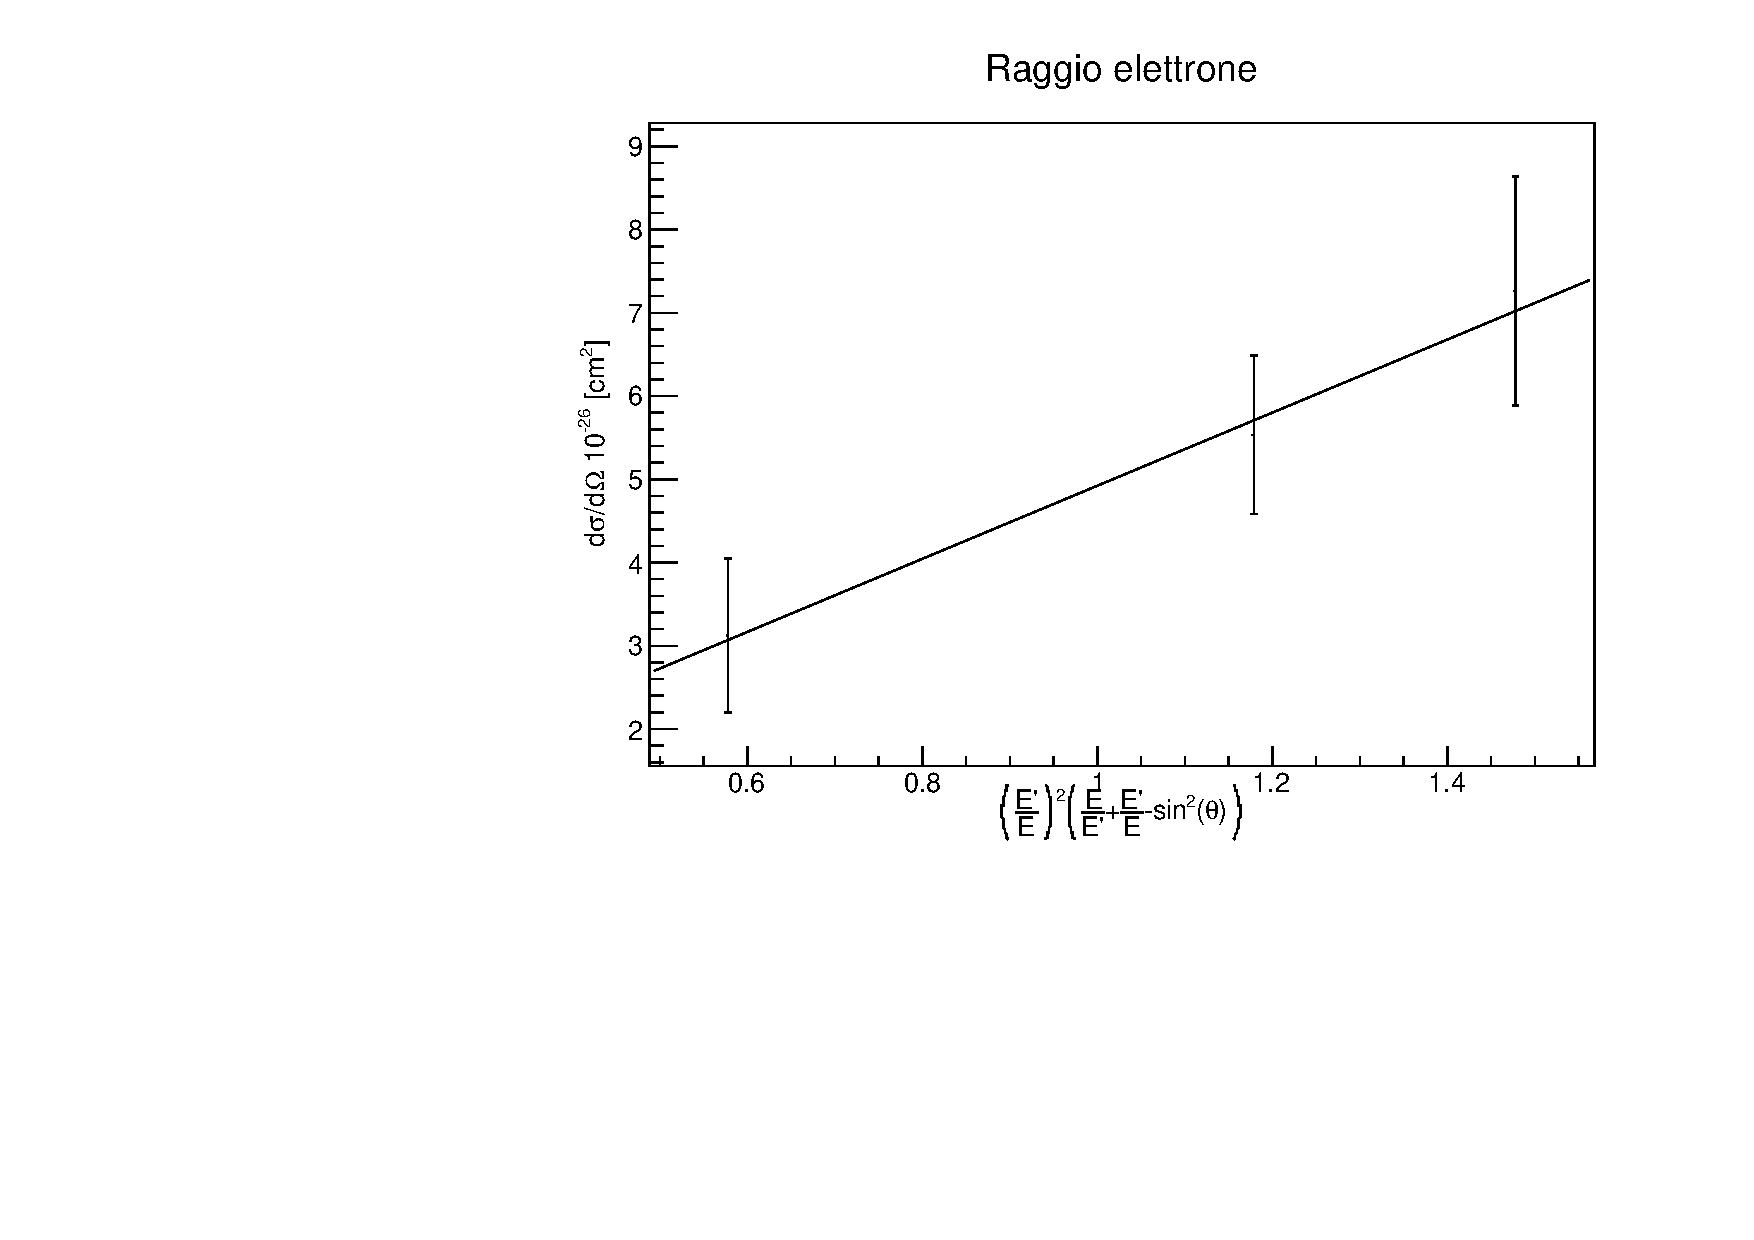
\includegraphics[width=12cm]{raggioelettrone.pdf}
\caption{Confronto tra andamento teorico (linea) e dati sperimentali per la misura del raggio dell'elettrone}
\end{figure}
La retta ottenuta ha un'equazione pari a EQUAZIONE, da cui si ricava un valore del raggio dell'elettrone pari a RAGGIO ELETTRONE, che RISULTA O NO  compatibile con il valore tabulato di $r_{e}$=2,82$\cdot10^{-13}$cm.


\chapter{Conclusioni}
In questa esperienza è stato possibile verificare la legge Compton e la legge Klein-Nishina, ottenendo andamenti dei dati compatibili con le previsioni teoriche. Il principale problema riscontrato è stato dato dai pochi dati raccolti per le misure: questo ha portato ad avere spettri che sono stati analizzati tutti in maniere differenti, a seconda delle diverse situazioni che si sono presentate, e ad errori percentuali piuttosto significativi. E' stato inoltre fondamentale prima della presa dati vera e propria ricalibrare l'apparato a seguito di un problema tecnico che ha portato ad una variazione della calibrazione precedentemente effettuata. Dai dati raccolti è stato inoltre possibile la misura della massa e del raggio dell'elettrone.





%%%----------------------------------------------------------
\MakeBibliography
%%%----------------------------------------------------------

\end{document}
